\documentclass[twoside]{book}

% Packages required by doxygen
\usepackage{fixltx2e}
\usepackage{calc}
\usepackage{doxygen}
\usepackage{graphicx}
\usepackage[utf8]{inputenc}
\usepackage{makeidx}
\usepackage{multicol}
\usepackage{multirow}
\PassOptionsToPackage{warn}{textcomp}
\usepackage{textcomp}
\usepackage[nointegrals]{wasysym}
\usepackage[table]{xcolor}

% Font selection
\usepackage[T1]{fontenc}
\usepackage{mathptmx}
\usepackage[scaled=.90]{helvet}
\usepackage{courier}
\usepackage{amssymb}
\usepackage{sectsty}
\renewcommand{\familydefault}{\sfdefault}
\allsectionsfont{%
  \fontseries{bc}\selectfont%
  \color{darkgray}%
}
\renewcommand{\DoxyLabelFont}{%
  \fontseries{bc}\selectfont%
  \color{darkgray}%
}
\newcommand{\+}{\discretionary{\mbox{\scriptsize$\hookleftarrow$}}{}{}}

% Page & text layout
\usepackage{geometry}
\geometry{%
  a4paper,%
  top=2.5cm,%
  bottom=2.5cm,%
  left=2.5cm,%
  right=2.5cm%
}
\tolerance=750
\hfuzz=15pt
\hbadness=750
\setlength{\emergencystretch}{15pt}
\setlength{\parindent}{0cm}
\setlength{\parskip}{0.2cm}
\makeatletter
\renewcommand{\paragraph}{%
  \@startsection{paragraph}{4}{0ex}{-1.0ex}{1.0ex}{%
    \normalfont\normalsize\bfseries\SS@parafont%
  }%
}
\renewcommand{\subparagraph}{%
  \@startsection{subparagraph}{5}{0ex}{-1.0ex}{1.0ex}{%
    \normalfont\normalsize\bfseries\SS@subparafont%
  }%
}
\makeatother

% Headers & footers
\usepackage{fancyhdr}
\pagestyle{fancyplain}
\fancyhead[LE]{\fancyplain{}{\bfseries\thepage}}
\fancyhead[CE]{\fancyplain{}{}}
\fancyhead[RE]{\fancyplain{}{\bfseries\leftmark}}
\fancyhead[LO]{\fancyplain{}{\bfseries\rightmark}}
\fancyhead[CO]{\fancyplain{}{}}
\fancyhead[RO]{\fancyplain{}{\bfseries\thepage}}
\fancyfoot[LE]{\fancyplain{}{}}
\fancyfoot[CE]{\fancyplain{}{}}
\fancyfoot[RE]{\fancyplain{}{\bfseries\scriptsize Generated on Sun Dec 20 2015 19\+:04\+:14 for Simulador de rede de Petri by Doxygen }}
\fancyfoot[LO]{\fancyplain{}{\bfseries\scriptsize Generated on Sun Dec 20 2015 19\+:04\+:14 for Simulador de rede de Petri by Doxygen }}
\fancyfoot[CO]{\fancyplain{}{}}
\fancyfoot[RO]{\fancyplain{}{}}
\renewcommand{\footrulewidth}{0.4pt}
\renewcommand{\chaptermark}[1]{%
  \markboth{#1}{}%
}
\renewcommand{\sectionmark}[1]{%
  \markright{\thesection\ #1}%
}

% Indices & bibliography
\usepackage{natbib}
\usepackage[titles]{tocloft}
\setcounter{tocdepth}{3}
\setcounter{secnumdepth}{5}
\makeindex

% Hyperlinks (required, but should be loaded last)
\usepackage{ifpdf}
\ifpdf
  \usepackage[pdftex,pagebackref=true]{hyperref}
\else
  \usepackage[ps2pdf,pagebackref=true]{hyperref}
\fi
\hypersetup{%
  colorlinks=true,%
  linkcolor=blue,%
  citecolor=blue,%
  unicode%
}

% Custom commands
\newcommand{\clearemptydoublepage}{%
  \newpage{\pagestyle{empty}\cleardoublepage}%
}


%===== C O N T E N T S =====

\begin{document}

% Titlepage & ToC
\hypersetup{pageanchor=false,
             bookmarks=true,
             bookmarksnumbered=true,
             pdfencoding=unicode
            }
\pagenumbering{roman}
\begin{titlepage}
\vspace*{7cm}
\begin{center}%
{\Large Simulador de rede de Petri \\[1ex]\large 2.\+0 }\\
\vspace*{1cm}
{\large Generated by Doxygen 1.8.8}\\
\vspace*{0.5cm}
{\small Sun Dec 20 2015 19:04:14}\\
\end{center}
\end{titlepage}
\clearemptydoublepage
\tableofcontents
\clearemptydoublepage
\pagenumbering{arabic}
\hypersetup{pageanchor=true}

%--- Begin generated contents ---
\chapter{Main Page}
\label{index}\hypertarget{index}{}\hyperlink{ex12_8c}{ex12.\+c} trata-\/se de uma simulação de uma rede de Petri, se utilizando dos recursos de dados abstratos e de threads. A entrada de dados será feita pela leitura dos valores nos arquivos entradas-\/petri.\+txt e os valores são armazena dos em variáveis, sendo os cinco primeiros valores representativos de quantidades (lugares, transições...), os demais não são variáveis únicas sendo necessário a utilização do sistema de lista para armazena-\/las. O paralelismo foi implementado para simular a aleatoriedade do programa, além de melhorar o processamento desta. Para cada thread haverá uma transição com listas de arcos que partem ou entram nela, denominadas listas de arco entram e de arco saem. Com base nessas listas arco é que a simulação funciona, retirando tokens, ativando transições e adicionando tokens em novos lugares ou no mesmo lugar. A rede de Petri é desenha para melhor visualização e para isso é utilizado a biblioteca allegro.\+h, na qual 3 funções derivam para desenhar tal rede, sendo elas (desenha\+\_\+estados, desenha\+\_\+transicao e desenha\+\_\+arcos).

\begin{DoxyVerb}Alunos: Arthur Carvalho de Albuquerque Cardoso
        Mateus Lenier Rezende
Professor: Dr. Ruben Carlo Benante.
Curso: Engenharia de Controle e Automação.\end{DoxyVerb}
 
\chapter{Data Structure Index}
\section{Data Structures}
Here are the data structures with brief descriptions\+:\begin{DoxyCompactList}
\item\contentsline{section}{\hyperlink{structst__arco}{st\+\_\+arco} \\*Struct utilizada na criação de duas listas\+: na lista de arco lugar-\/transição e na lista de transição-\/lugar }{\pageref{structst__arco}}{}
\item\contentsline{section}{\hyperlink{structst__lugartoken}{st\+\_\+lugartoken} \\*Struct utilizada no armazenamento da quantidade de tokens em função do lugar }{\pageref{structst__lugartoken}}{}
\item\contentsline{section}{\hyperlink{structst__thread}{st\+\_\+thread} \\*Struct utilizada na criação de uma lista pthread }{\pageref{structst__thread}}{}
\item\contentsline{section}{\hyperlink{structst__transicao}{st\+\_\+transicao} \\*Struct utilizada na criação de uma lista de transições e que tambem possui duas listas, de arcos que entram e que saem da transição }{\pageref{structst__transicao}}{}
\end{DoxyCompactList}

\chapter{File Index}
\section{File List}
Here is a list of all files with brief descriptions\+:\begin{DoxyCompactList}
\item\contentsline{section}{\hyperlink{ex12_8c}{ex12.\+c} \\*Simulador de rede de petri }{\pageref{ex12_8c}}{}
\end{DoxyCompactList}

\chapter{Data Structure Documentation}
\hypertarget{structst__arco}{\section{st\+\_\+arco Struct Reference}
\label{structst__arco}\index{st\+\_\+arco@{st\+\_\+arco}}
}


Struct utilizada na criação de duas listas\+: na lista de arco lugar-\/transição e na lista de transição-\/lugar.  




Collaboration diagram for st\+\_\+arco\+:\nopagebreak
\begin{figure}[H]
\begin{center}
\leavevmode
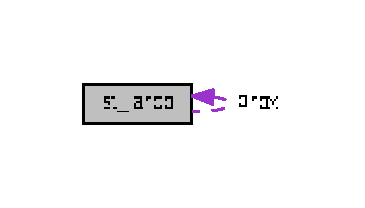
\includegraphics[width=175pt]{structst__arco__coll__graph}
\end{center}
\end{figure}
\subsection*{Data Fields}
\begin{DoxyCompactItemize}
\item 
int \hyperlink{structst__arco_a640a8b25b7f08e94cc6e535523aa8857}{inicio}
\item 
int \hyperlink{structst__arco_aa9099d2432e77829a68e2aacea614b57}{tkgp}
\item 
int \hyperlink{structst__arco_a2215b7a64f0bc19a8916059b80a8a7e4}{final}
\item 
struct \hyperlink{structst__arco}{st\+\_\+arco} $\ast$ \hyperlink{structst__arco_a7e122db30f69e19aed8a7ce0295920c0}{prox}
\end{DoxyCompactItemize}


\subsection{Detailed Description}
Struct utilizada na criação de duas listas\+: na lista de arco lugar-\/transição e na lista de transição-\/lugar. 



Definition at line 85 of file ex12.\+c.



\subsection{Field Documentation}
\hypertarget{structst__arco_a2215b7a64f0bc19a8916059b80a8a7e4}{\index{st\+\_\+arco@{st\+\_\+arco}!final@{final}}
\index{final@{final}!st\+\_\+arco@{st\+\_\+arco}}
\subsubsection[{final}]{\setlength{\rightskip}{0pt plus 5cm}int st\+\_\+arco\+::final}}\label{structst__arco_a2215b7a64f0bc19a8916059b80a8a7e4}


Definition at line 87 of file ex12.\+c.

\hypertarget{structst__arco_a640a8b25b7f08e94cc6e535523aa8857}{\index{st\+\_\+arco@{st\+\_\+arco}!inicio@{inicio}}
\index{inicio@{inicio}!st\+\_\+arco@{st\+\_\+arco}}
\subsubsection[{inicio}]{\setlength{\rightskip}{0pt plus 5cm}int st\+\_\+arco\+::inicio}}\label{structst__arco_a640a8b25b7f08e94cc6e535523aa8857}


Definition at line 87 of file ex12.\+c.

\hypertarget{structst__arco_a7e122db30f69e19aed8a7ce0295920c0}{\index{st\+\_\+arco@{st\+\_\+arco}!prox@{prox}}
\index{prox@{prox}!st\+\_\+arco@{st\+\_\+arco}}
\subsubsection[{prox}]{\setlength{\rightskip}{0pt plus 5cm}struct {\bf st\+\_\+arco}$\ast$ st\+\_\+arco\+::prox}}\label{structst__arco_a7e122db30f69e19aed8a7ce0295920c0}


Definition at line 88 of file ex12.\+c.

\hypertarget{structst__arco_aa9099d2432e77829a68e2aacea614b57}{\index{st\+\_\+arco@{st\+\_\+arco}!tkgp@{tkgp}}
\index{tkgp@{tkgp}!st\+\_\+arco@{st\+\_\+arco}}
\subsubsection[{tkgp}]{\setlength{\rightskip}{0pt plus 5cm}int st\+\_\+arco\+::tkgp}}\label{structst__arco_aa9099d2432e77829a68e2aacea614b57}


Definition at line 87 of file ex12.\+c.



The documentation for this struct was generated from the following file\+:\begin{DoxyCompactItemize}
\item 
\hyperlink{ex12_8c}{ex12.\+c}\end{DoxyCompactItemize}

\hypertarget{structst__lugartoken}{\section{st\+\_\+lugartoken Struct Reference}
\label{structst__lugartoken}\index{st\+\_\+lugartoken@{st\+\_\+lugartoken}}
}


Struct utilizada no armazenamento da quantidade de tokens em função do lugar.  




Collaboration diagram for st\+\_\+lugartoken\+:\nopagebreak
\begin{figure}[H]
\begin{center}
\leavevmode
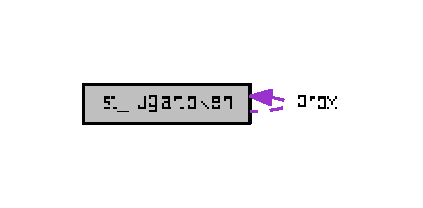
\includegraphics[width=203pt]{structst__lugartoken__coll__graph}
\end{center}
\end{figure}
\subsection*{Data Fields}
\begin{DoxyCompactItemize}
\item 
int \hyperlink{structst__lugartoken_aa0ef964380839df33cf936fdc0bfdf66}{lu}
\item 
int \hyperlink{structst__lugartoken_a58b3c1ed10063127a3f50aefa336250c}{tk}
\item 
struct \hyperlink{structst__lugartoken}{st\+\_\+lugartoken} $\ast$ \hyperlink{structst__lugartoken_a274f4c1422ff1d2c56e58495734b4bc3}{prox}
\end{DoxyCompactItemize}


\subsection{Detailed Description}
Struct utilizada no armazenamento da quantidade de tokens em função do lugar. 



Definition at line 100 of file ex12.\+c.



\subsection{Field Documentation}
\hypertarget{structst__lugartoken_aa0ef964380839df33cf936fdc0bfdf66}{\index{st\+\_\+lugartoken@{st\+\_\+lugartoken}!lu@{lu}}
\index{lu@{lu}!st\+\_\+lugartoken@{st\+\_\+lugartoken}}
\subsubsection[{lu}]{\setlength{\rightskip}{0pt plus 5cm}int st\+\_\+lugartoken\+::lu}}\label{structst__lugartoken_aa0ef964380839df33cf936fdc0bfdf66}


Definition at line 102 of file ex12.\+c.

\hypertarget{structst__lugartoken_a274f4c1422ff1d2c56e58495734b4bc3}{\index{st\+\_\+lugartoken@{st\+\_\+lugartoken}!prox@{prox}}
\index{prox@{prox}!st\+\_\+lugartoken@{st\+\_\+lugartoken}}
\subsubsection[{prox}]{\setlength{\rightskip}{0pt plus 5cm}struct {\bf st\+\_\+lugartoken}$\ast$ st\+\_\+lugartoken\+::prox}}\label{structst__lugartoken_a274f4c1422ff1d2c56e58495734b4bc3}


Definition at line 103 of file ex12.\+c.

\hypertarget{structst__lugartoken_a58b3c1ed10063127a3f50aefa336250c}{\index{st\+\_\+lugartoken@{st\+\_\+lugartoken}!tk@{tk}}
\index{tk@{tk}!st\+\_\+lugartoken@{st\+\_\+lugartoken}}
\subsubsection[{tk}]{\setlength{\rightskip}{0pt plus 5cm}int st\+\_\+lugartoken\+::tk}}\label{structst__lugartoken_a58b3c1ed10063127a3f50aefa336250c}


Definition at line 102 of file ex12.\+c.



The documentation for this struct was generated from the following file\+:\begin{DoxyCompactItemize}
\item 
\hyperlink{ex12_8c}{ex12.\+c}\end{DoxyCompactItemize}

\hypertarget{structst__thread}{\section{st\+\_\+thread Struct Reference}
\label{structst__thread}\index{st\+\_\+thread@{st\+\_\+thread}}
}


Struct utilizada na criação de uma lista pthread.  




Collaboration diagram for st\+\_\+thread\+:\nopagebreak
\begin{figure}[H]
\begin{center}
\leavevmode
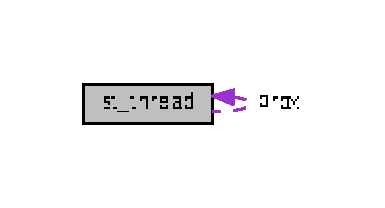
\includegraphics[width=185pt]{structst__thread__coll__graph}
\end{center}
\end{figure}
\subsection*{Data Fields}
\begin{DoxyCompactItemize}
\item 
pthread\+\_\+t \hyperlink{structst__thread_a33fbd41433c488aeecd687625196d115}{thr}
\item 
struct \hyperlink{structst__thread}{st\+\_\+thread} $\ast$ \hyperlink{structst__thread_aa4a7a171525a32aa2e9244112bfc0889}{prox}
\end{DoxyCompactItemize}


\subsection{Detailed Description}
Struct utilizada na criação de uma lista pthread. 



Definition at line 79 of file ex12.\+c.



\subsection{Field Documentation}
\hypertarget{structst__thread_aa4a7a171525a32aa2e9244112bfc0889}{\index{st\+\_\+thread@{st\+\_\+thread}!prox@{prox}}
\index{prox@{prox}!st\+\_\+thread@{st\+\_\+thread}}
\subsubsection[{prox}]{\setlength{\rightskip}{0pt plus 5cm}struct {\bf st\+\_\+thread}$\ast$ st\+\_\+thread\+::prox}}\label{structst__thread_aa4a7a171525a32aa2e9244112bfc0889}


Definition at line 82 of file ex12.\+c.

\hypertarget{structst__thread_a33fbd41433c488aeecd687625196d115}{\index{st\+\_\+thread@{st\+\_\+thread}!thr@{thr}}
\index{thr@{thr}!st\+\_\+thread@{st\+\_\+thread}}
\subsubsection[{thr}]{\setlength{\rightskip}{0pt plus 5cm}pthread\+\_\+t st\+\_\+thread\+::thr}}\label{structst__thread_a33fbd41433c488aeecd687625196d115}


Definition at line 81 of file ex12.\+c.



The documentation for this struct was generated from the following file\+:\begin{DoxyCompactItemize}
\item 
\hyperlink{ex12_8c}{ex12.\+c}\end{DoxyCompactItemize}

\hypertarget{structst__transicao}{\section{st\+\_\+transicao Struct Reference}
\label{structst__transicao}\index{st\+\_\+transicao@{st\+\_\+transicao}}
}


Struct utilizada na criação de uma lista de transições e que tambem possui duas listas, de arcos que entram e que saem da transição.  




Collaboration diagram for st\+\_\+transicao\+:\nopagebreak
\begin{figure}[H]
\begin{center}
\leavevmode
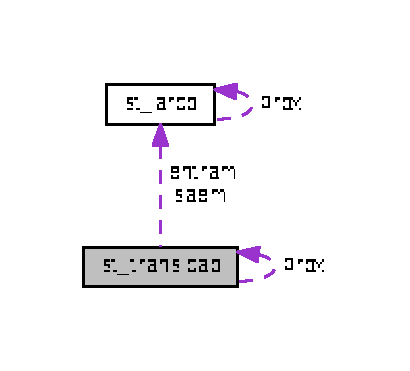
\includegraphics[width=197pt]{structst__transicao__coll__graph}
\end{center}
\end{figure}
\subsection*{Data Fields}
\begin{DoxyCompactItemize}
\item 
int \hyperlink{structst__transicao_a22bd0f442dc1aaab89357adf10199cc2}{trans}
\item 
\hyperlink{ex12_8c_a903d87a3126ea1585f84d7cdf488c4a3}{arco} $\ast$ \hyperlink{structst__transicao_ac6c32a5c66564a64d08f8236fbd8f0cb}{entram}
\item 
\hyperlink{ex12_8c_a903d87a3126ea1585f84d7cdf488c4a3}{arco} $\ast$ \hyperlink{structst__transicao_ad8423428e8e7544bbed187f4a78b11ab}{saem}
\item 
struct \hyperlink{structst__transicao}{st\+\_\+transicao} $\ast$ \hyperlink{structst__transicao_a48dfc1e8eb0e9d01877112b340d7ba5c}{prox}
\end{DoxyCompactItemize}


\subsection{Detailed Description}
Struct utilizada na criação de uma lista de transições e que tambem possui duas listas, de arcos que entram e que saem da transição. 



Definition at line 91 of file ex12.\+c.



\subsection{Field Documentation}
\hypertarget{structst__transicao_ac6c32a5c66564a64d08f8236fbd8f0cb}{\index{st\+\_\+transicao@{st\+\_\+transicao}!entram@{entram}}
\index{entram@{entram}!st\+\_\+transicao@{st\+\_\+transicao}}
\subsubsection[{entram}]{\setlength{\rightskip}{0pt plus 5cm}{\bf arco}$\ast$ st\+\_\+transicao\+::entram}}\label{structst__transicao_ac6c32a5c66564a64d08f8236fbd8f0cb}


Definition at line 94 of file ex12.\+c.

\hypertarget{structst__transicao_a48dfc1e8eb0e9d01877112b340d7ba5c}{\index{st\+\_\+transicao@{st\+\_\+transicao}!prox@{prox}}
\index{prox@{prox}!st\+\_\+transicao@{st\+\_\+transicao}}
\subsubsection[{prox}]{\setlength{\rightskip}{0pt plus 5cm}struct {\bf st\+\_\+transicao}$\ast$ st\+\_\+transicao\+::prox}}\label{structst__transicao_a48dfc1e8eb0e9d01877112b340d7ba5c}


Definition at line 96 of file ex12.\+c.

\hypertarget{structst__transicao_ad8423428e8e7544bbed187f4a78b11ab}{\index{st\+\_\+transicao@{st\+\_\+transicao}!saem@{saem}}
\index{saem@{saem}!st\+\_\+transicao@{st\+\_\+transicao}}
\subsubsection[{saem}]{\setlength{\rightskip}{0pt plus 5cm}{\bf arco}$\ast$ st\+\_\+transicao\+::saem}}\label{structst__transicao_ad8423428e8e7544bbed187f4a78b11ab}


Definition at line 95 of file ex12.\+c.

\hypertarget{structst__transicao_a22bd0f442dc1aaab89357adf10199cc2}{\index{st\+\_\+transicao@{st\+\_\+transicao}!trans@{trans}}
\index{trans@{trans}!st\+\_\+transicao@{st\+\_\+transicao}}
\subsubsection[{trans}]{\setlength{\rightskip}{0pt plus 5cm}int st\+\_\+transicao\+::trans}}\label{structst__transicao_a22bd0f442dc1aaab89357adf10199cc2}


Definition at line 93 of file ex12.\+c.



The documentation for this struct was generated from the following file\+:\begin{DoxyCompactItemize}
\item 
\hyperlink{ex12_8c}{ex12.\+c}\end{DoxyCompactItemize}

\chapter{File Documentation}
\hypertarget{ex12_8c}{\section{ex12.\+c File Reference}
\label{ex12_8c}\index{ex12.\+c@{ex12.\+c}}
}


simulador de rede de petri  


Include dependency graph for ex12.\+c\+:\nopagebreak
\begin{figure}[H]
\begin{center}
\leavevmode
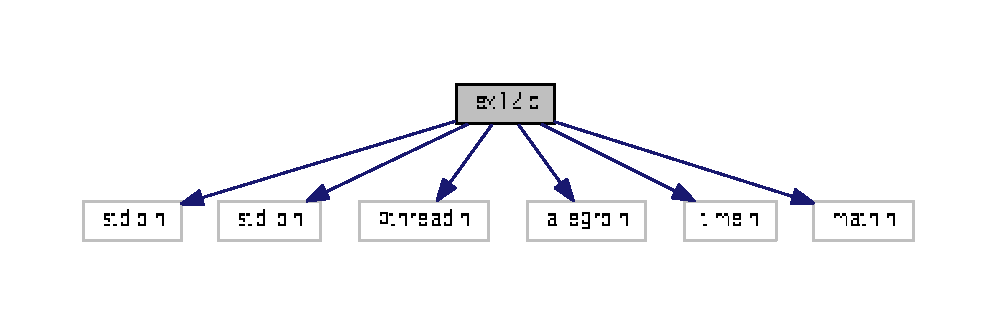
\includegraphics[width=350pt]{ex12_8c__incl}
\end{center}
\end{figure}
\subsection*{Data Structures}
\begin{DoxyCompactItemize}
\item 
struct \hyperlink{structst__thread}{st\+\_\+thread}
\begin{DoxyCompactList}\small\item\em Struct utilizada na criação de uma lista pthread. \end{DoxyCompactList}\item 
struct \hyperlink{structst__arco}{st\+\_\+arco}
\begin{DoxyCompactList}\small\item\em Struct utilizada na criação de duas listas\+: na lista de arco lugar-\/transição e na lista de transição-\/lugar. \end{DoxyCompactList}\item 
struct \hyperlink{structst__transicao}{st\+\_\+transicao}
\begin{DoxyCompactList}\small\item\em Struct utilizada na criação de uma lista de transições e que tambem possui duas listas, de arcos que entram e que saem da transição. \end{DoxyCompactList}\item 
struct \hyperlink{structst__lugartoken}{st\+\_\+lugartoken}
\begin{DoxyCompactList}\small\item\em Struct utilizada no armazenamento da quantidade de tokens em função do lugar. \end{DoxyCompactList}\end{DoxyCompactItemize}
\subsection*{Macros}
\begin{DoxyCompactItemize}
\item 
\#define \hyperlink{ex12_8c_afd7feb39acd312085566c208e35c2362}{F\+N\+A\+M\+E}~\char`\"{}entrada-\/petri-\/1.txt\char`\"{}
\begin{DoxyCompactList}\small\item\em Entrada de dados. \end{DoxyCompactList}\item 
\#define \hyperlink{ex12_8c_a35243471650921a66d36df618019c9d9}{V\+A\+Z\+I\+O}~0
\begin{DoxyCompactList}\small\item\em Define para nao ter numero magico, caso lugar com 0 token. \end{DoxyCompactList}\item 
\#define \hyperlink{ex12_8c_a207fd5507206d307cd63f95374fcd00d}{X}~800
\begin{DoxyCompactList}\small\item\em Tamanho X da tela. \end{DoxyCompactList}\item 
\#define \hyperlink{ex12_8c_a798e4073d613ca5ba9618e1b3253df14}{Y}~600
\begin{DoxyCompactList}\small\item\em Tamanho Y da tela. \end{DoxyCompactList}\item 
\#define \hyperlink{ex12_8c_afbdf6aaa9dc9536814753a2676ae503e}{X\+Centro}~\hyperlink{ex12_8c_a207fd5507206d307cd63f95374fcd00d}{X}/2.\+0
\begin{DoxyCompactList}\small\item\em Posicao X do centro da circunferencia. \end{DoxyCompactList}\item 
\#define \hyperlink{ex12_8c_a56ca31f80a4aa2287e297e7f9f2530ae}{Y\+Centro}~\hyperlink{ex12_8c_a798e4073d613ca5ba9618e1b3253df14}{Y}/2.\+0
\begin{DoxyCompactList}\small\item\em Posicao Y do centro da circunferencia. \end{DoxyCompactList}\item 
\#define \hyperlink{ex12_8c_a3fa02c0d4875f25146e01888e683baaa}{I\+M\+A\+G\+E\+N\+A\+M\+E}~\char`\"{}ex12.\+bmp\char`\"{}
\begin{DoxyCompactList}\small\item\em Imagem gerada pelo allegro. \end{DoxyCompactList}\item 
\#define \hyperlink{ex12_8c_a564a8a1173bd4fb63c4f3a1903143e6a}{C\+O\+R\+B\+R\+A\+N\+C\+O}~(makecol(255,255,255))
\begin{DoxyCompactList}\small\item\em Macro para cor branca. \end{DoxyCompactList}\item 
\#define \hyperlink{ex12_8c_aaa9af825d3a4f75b40c0403bd37c55bd}{C\+O\+R\+P\+R\+E\+T\+O}~1
\begin{DoxyCompactList}\small\item\em Macro para cor preta. \end{DoxyCompactList}\item 
\#define \hyperlink{ex12_8c_a6ba7276f7e11d0099ad5386922bfa495}{C\+O\+R\+C\+I\+N\+Z\+A}~(makecol(160,160,160))
\begin{DoxyCompactList}\small\item\em Macro para cor cinza. \end{DoxyCompactList}\item 
\#define \hyperlink{ex12_8c_a70d9bb57e73b641e6394d1a743d4d891}{C\+O\+R\+A\+Z\+U\+L}~(makecol(0,0,255))
\begin{DoxyCompactList}\small\item\em Macro para cor azul. \end{DoxyCompactList}\item 
\#define \hyperlink{ex12_8c_ad7dde6e35154225591228222edb21c1b}{C\+O\+R\+V\+E\+R\+D\+E}~(makecol(0,255,0))
\begin{DoxyCompactList}\small\item\em Macro para cor verde. \end{DoxyCompactList}\item 
\#define \hyperlink{ex12_8c_a70bb1aad71a6f756c61983e9fa967737}{C\+O\+R\+A\+M\+A\+R\+E\+L\+O}~(makecol(255,255,100))
\begin{DoxyCompactList}\small\item\em Macro para cor amarelo. \end{DoxyCompactList}\item 
\#define \hyperlink{ex12_8c_a0e2857429e52d86533c9fcc6b7e92bfb}{C\+O\+R\+V\+E\+R\+M\+E\+L\+H\+O}~(makecol(255,0,0))
\begin{DoxyCompactList}\small\item\em Macro para cor vermelho. \end{DoxyCompactList}\item 
\#define \hyperlink{ex12_8c_a5de5d183f9a6a8d53316f743e1ca6dc2}{N\+M\+A\+X}~1000
\begin{DoxyCompactList}\small\item\em Numero de interacoes petri. \end{DoxyCompactList}\item 
\#define \hyperlink{ex12_8c_ac257b1448c6f4ba1ffc7d2c1fd1e5514}{P\+A\+T}~50
\begin{DoxyCompactList}\small\item\em Porcentagem de ativacao da transicao. \end{DoxyCompactList}\item 
\#define \hyperlink{ex12_8c_ad72dbcf6d0153db1b8d8a58001feed83}{D\+E\+B\+U\+G}~0
\begin{DoxyCompactList}\small\item\em Ativa D\+E\+B\+U\+G. \end{DoxyCompactList}\end{DoxyCompactItemize}
\subsection*{Typedefs}
\begin{DoxyCompactItemize}
\item 
typedef struct \hyperlink{structst__thread}{st\+\_\+thread} \hyperlink{ex12_8c_a019c873b87fedc4700c93daa592d5c7c}{thread}
\begin{DoxyCompactList}\small\item\em Struct utilizada na criação de uma lista pthread. \end{DoxyCompactList}\item 
typedef struct \hyperlink{structst__arco}{st\+\_\+arco} \hyperlink{ex12_8c_a903d87a3126ea1585f84d7cdf488c4a3}{arco}
\begin{DoxyCompactList}\small\item\em Struct utilizada na criação de duas listas\+: na lista de arco lugar-\/transição e na lista de transição-\/lugar. \end{DoxyCompactList}\item 
typedef struct \hyperlink{structst__transicao}{st\+\_\+transicao} \hyperlink{ex12_8c_ab2ead25480371ac5fb59d5d03baf6a3c}{transicao}
\begin{DoxyCompactList}\small\item\em Struct utilizada na criação de uma lista de transições e que tambem possui duas listas, de arcos que entram e que saem da transição. \end{DoxyCompactList}\item 
typedef struct \hyperlink{structst__lugartoken}{st\+\_\+lugartoken} \hyperlink{ex12_8c_a9e1493b8a046b2476b7fa548b55cc3da}{lugartoken}
\begin{DoxyCompactList}\small\item\em Struct utilizada no armazenamento da quantidade de tokens em função do lugar. \end{DoxyCompactList}\end{DoxyCompactItemize}
\subsection*{Functions}
\begin{DoxyCompactItemize}
\item 
void $\ast$ \hyperlink{ex12_8c_a3abecd9a7dc3f7aaeac7406c356268d0}{simupetri} (void $\ast$trtemp)
\begin{DoxyCompactList}\small\item\em Função para simular a rede de petri. \end{DoxyCompactList}\item 
void \hyperlink{ex12_8c_a497fc35896bf4023d3b96caf1f5a905a}{inserirlutk} (\hyperlink{ex12_8c_a9e1493b8a046b2476b7fa548b55cc3da}{lugartoken} $\ast$$\ast$cabeca, int lu, int tk)
\begin{DoxyCompactList}\small\item\em Função para inserir novos lugarestokens na lista. \end{DoxyCompactList}\item 
void \hyperlink{ex12_8c_a24cf4210cd09450432e9e537d66ed120}{inserirtransicao} (\hyperlink{ex12_8c_ab2ead25480371ac5fb59d5d03baf6a3c}{transicao} $\ast$$\ast$cabeca, int i)
\begin{DoxyCompactList}\small\item\em Função para inserir novas transições na lista. \end{DoxyCompactList}\item 
void \hyperlink{ex12_8c_aaa991ba94684a02e8e12d6a343635731}{inserirentram} (\hyperlink{ex12_8c_a903d87a3126ea1585f84d7cdf488c4a3}{arco} $\ast$$\ast$cabeca, int inicio, int tkgp, int final)
\begin{DoxyCompactList}\small\item\em Função para inserir novas transições na lista. \end{DoxyCompactList}\item 
void \hyperlink{ex12_8c_a360df5d24e27980134de470cb437eac7}{inserirpthread} (\hyperlink{ex12_8c_a019c873b87fedc4700c93daa592d5c7c}{thread} $\ast$$\ast$cabeca, pthread\+\_\+t p)
\begin{DoxyCompactList}\small\item\em Função para inserir novos arcos na lista, tanto arco lugar-\/transição quanto transição-\/lugar. \end{DoxyCompactList}\item 
void \hyperlink{ex12_8c_a0f0d38457a8e40bc4cc2dafe5318950e}{ativacaotransicao} (\hyperlink{ex12_8c_a903d87a3126ea1585f84d7cdf488c4a3}{arco} $\ast$head, \hyperlink{ex12_8c_a9e1493b8a046b2476b7fa548b55cc3da}{lugartoken} $\ast$$\ast$cabeca)
\begin{DoxyCompactList}\small\item\em Função para inserir novas pthreads na lista. \end{DoxyCompactList}\item 
void \hyperlink{ex12_8c_a6425f3c78a19798db5e3078d6a63ff69}{retiratoken} (\hyperlink{ex12_8c_a9e1493b8a046b2476b7fa548b55cc3da}{lugartoken} $\ast$$\ast$cabeca, \hyperlink{ex12_8c_a903d87a3126ea1585f84d7cdf488c4a3}{arco} $\ast$head, \hyperlink{ex12_8c_a903d87a3126ea1585f84d7cdf488c4a3}{arco} $\ast$kopf)
\begin{DoxyCompactList}\small\item\em Função que simula a ativação das transiçôes na rede de petri. \end{DoxyCompactList}\item 
void \hyperlink{ex12_8c_a7910bdb88a9403463674c9e4aaa90f77}{gerar\+\_\+imagem} (\hyperlink{ex12_8c_ab2ead25480371ac5fb59d5d03baf6a3c}{transicao} $\ast$tr, int ql, int qt)
\begin{DoxyCompactList}\small\item\em Função utilizada para desenhar a rede de petri utilizando a biblioteca do allegro. \end{DoxyCompactList}\item 
void \hyperlink{ex12_8c_a2adadcc2b98c8447fe423df994e5ab49}{desenha\+\_\+estados} (B\+I\+T\+M\+A\+P $\ast$buff, int k)
\begin{DoxyCompactList}\small\item\em Função utilizada para desenhar a rede de petri utilizando a biblioteca do allegro. \end{DoxyCompactList}\item 
void \hyperlink{ex12_8c_a3584be4f301e68bc12074b09f874ded5}{desenha\+\_\+transicoes} (B\+I\+T\+M\+A\+P $\ast$buff, \hyperlink{ex12_8c_ab2ead25480371ac5fb59d5d03baf6a3c}{transicao} $\ast$trans, int k, int c)
\begin{DoxyCompactList}\small\item\em Função para desenhar os lugares da rede de petri. \end{DoxyCompactList}\item 
void \hyperlink{ex12_8c_a93fe8b90c69f52c49c86ccc1d6df7e29}{desenha\+\_\+arcos} (int qo, int qf, B\+I\+T\+M\+A\+P $\ast$buff, int k, int c, int flag)
\begin{DoxyCompactList}\small\item\em Função para desenhar as transições da rede de petri. \end{DoxyCompactList}\item 
float \hyperlink{ex12_8c_aa860d66cac524ebe1f6d58074fc9e631}{alsin} (float x1, float y1, float x2, float y2)
\begin{DoxyCompactList}\small\item\em Funções utilizadas para desenhar os arcos da rede de petri. \end{DoxyCompactList}\item 
float \hyperlink{ex12_8c_a6531e2583fdd9a9198526cdd2ac38ce5}{alcos} (float x1, float y1, float x2, float y2)
\begin{DoxyCompactList}\small\item\em Função que calcula um seno que será utilizado no desenho da seta. \end{DoxyCompactList}\item 
float \hyperlink{ex12_8c_af4699181d7bf8a6ccce6902827c9b975}{arctan} (float x1, float y1, float x2, float y2)
\begin{DoxyCompactList}\small\item\em Função que calcula um cosseno que será utilizado no desenho da seta. \end{DoxyCompactList}\item 
int \hyperlink{ex12_8c_a840291bc02cba5474a4cb46a9b9566fe}{main} (void)
\begin{DoxyCompactList}\small\item\em Função que calcula o arcotangente para todos os quadrantes de forma individual. \end{DoxyCompactList}\end{DoxyCompactItemize}
\subsection*{Variables}
\begin{DoxyCompactItemize}
\item 
static struct \hyperlink{structst__lugartoken}{st\+\_\+lugartoken} $\ast$ \hyperlink{ex12_8c_ad6d55b93bce67d30cc6672b642fd4602}{lntk}
\end{DoxyCompactItemize}


\subsection{Detailed Description}
simulador de rede de petri 

\begin{DoxyAuthor}{Author}
Arthur Carvalho de Albuquerque Cardoso $<$\href{mailto:arthurcardoso2005@hotmail.com}{\tt arthurcardoso2005@hotmail.\+com}$>$ 

Mateus Lenier Rezende $<$\href{mailto:mateuslenier@gmail.com}{\tt mateuslenier@gmail.\+com}$>$ 
\end{DoxyAuthor}
\begin{DoxyVersion}{Version}
2.\+0 
\end{DoxyVersion}
\begin{DoxyDate}{Date}
2015-\/12-\/20 
\end{DoxyDate}


Definition in file \hyperlink{ex12_8c_source}{ex12.\+c}.



\subsection{Macro Definition Documentation}
\hypertarget{ex12_8c_a70bb1aad71a6f756c61983e9fa967737}{\index{ex12.\+c@{ex12.\+c}!C\+O\+R\+A\+M\+A\+R\+E\+L\+O@{C\+O\+R\+A\+M\+A\+R\+E\+L\+O}}
\index{C\+O\+R\+A\+M\+A\+R\+E\+L\+O@{C\+O\+R\+A\+M\+A\+R\+E\+L\+O}!ex12.\+c@{ex12.\+c}}
\subsubsection[{C\+O\+R\+A\+M\+A\+R\+E\+L\+O}]{\setlength{\rightskip}{0pt plus 5cm}\#define C\+O\+R\+A\+M\+A\+R\+E\+L\+O~(makecol(255,255,100))}}\label{ex12_8c_a70bb1aad71a6f756c61983e9fa967737}


Macro para cor amarelo. 



Definition at line 64 of file ex12.\+c.

\hypertarget{ex12_8c_a70d9bb57e73b641e6394d1a743d4d891}{\index{ex12.\+c@{ex12.\+c}!C\+O\+R\+A\+Z\+U\+L@{C\+O\+R\+A\+Z\+U\+L}}
\index{C\+O\+R\+A\+Z\+U\+L@{C\+O\+R\+A\+Z\+U\+L}!ex12.\+c@{ex12.\+c}}
\subsubsection[{C\+O\+R\+A\+Z\+U\+L}]{\setlength{\rightskip}{0pt plus 5cm}\#define C\+O\+R\+A\+Z\+U\+L~(makecol(0,0,255))}}\label{ex12_8c_a70d9bb57e73b641e6394d1a743d4d891}


Macro para cor azul. 



Definition at line 62 of file ex12.\+c.

\hypertarget{ex12_8c_a564a8a1173bd4fb63c4f3a1903143e6a}{\index{ex12.\+c@{ex12.\+c}!C\+O\+R\+B\+R\+A\+N\+C\+O@{C\+O\+R\+B\+R\+A\+N\+C\+O}}
\index{C\+O\+R\+B\+R\+A\+N\+C\+O@{C\+O\+R\+B\+R\+A\+N\+C\+O}!ex12.\+c@{ex12.\+c}}
\subsubsection[{C\+O\+R\+B\+R\+A\+N\+C\+O}]{\setlength{\rightskip}{0pt plus 5cm}\#define C\+O\+R\+B\+R\+A\+N\+C\+O~(makecol(255,255,255))}}\label{ex12_8c_a564a8a1173bd4fb63c4f3a1903143e6a}


Macro para cor branca. 



Definition at line 59 of file ex12.\+c.

\hypertarget{ex12_8c_a6ba7276f7e11d0099ad5386922bfa495}{\index{ex12.\+c@{ex12.\+c}!C\+O\+R\+C\+I\+N\+Z\+A@{C\+O\+R\+C\+I\+N\+Z\+A}}
\index{C\+O\+R\+C\+I\+N\+Z\+A@{C\+O\+R\+C\+I\+N\+Z\+A}!ex12.\+c@{ex12.\+c}}
\subsubsection[{C\+O\+R\+C\+I\+N\+Z\+A}]{\setlength{\rightskip}{0pt plus 5cm}\#define C\+O\+R\+C\+I\+N\+Z\+A~(makecol(160,160,160))}}\label{ex12_8c_a6ba7276f7e11d0099ad5386922bfa495}


Macro para cor cinza. 



Definition at line 61 of file ex12.\+c.

\hypertarget{ex12_8c_aaa9af825d3a4f75b40c0403bd37c55bd}{\index{ex12.\+c@{ex12.\+c}!C\+O\+R\+P\+R\+E\+T\+O@{C\+O\+R\+P\+R\+E\+T\+O}}
\index{C\+O\+R\+P\+R\+E\+T\+O@{C\+O\+R\+P\+R\+E\+T\+O}!ex12.\+c@{ex12.\+c}}
\subsubsection[{C\+O\+R\+P\+R\+E\+T\+O}]{\setlength{\rightskip}{0pt plus 5cm}\#define C\+O\+R\+P\+R\+E\+T\+O~1}}\label{ex12_8c_aaa9af825d3a4f75b40c0403bd37c55bd}


Macro para cor preta. 



Definition at line 60 of file ex12.\+c.

\hypertarget{ex12_8c_ad7dde6e35154225591228222edb21c1b}{\index{ex12.\+c@{ex12.\+c}!C\+O\+R\+V\+E\+R\+D\+E@{C\+O\+R\+V\+E\+R\+D\+E}}
\index{C\+O\+R\+V\+E\+R\+D\+E@{C\+O\+R\+V\+E\+R\+D\+E}!ex12.\+c@{ex12.\+c}}
\subsubsection[{C\+O\+R\+V\+E\+R\+D\+E}]{\setlength{\rightskip}{0pt plus 5cm}\#define C\+O\+R\+V\+E\+R\+D\+E~(makecol(0,255,0))}}\label{ex12_8c_ad7dde6e35154225591228222edb21c1b}


Macro para cor verde. 



Definition at line 63 of file ex12.\+c.

\hypertarget{ex12_8c_a0e2857429e52d86533c9fcc6b7e92bfb}{\index{ex12.\+c@{ex12.\+c}!C\+O\+R\+V\+E\+R\+M\+E\+L\+H\+O@{C\+O\+R\+V\+E\+R\+M\+E\+L\+H\+O}}
\index{C\+O\+R\+V\+E\+R\+M\+E\+L\+H\+O@{C\+O\+R\+V\+E\+R\+M\+E\+L\+H\+O}!ex12.\+c@{ex12.\+c}}
\subsubsection[{C\+O\+R\+V\+E\+R\+M\+E\+L\+H\+O}]{\setlength{\rightskip}{0pt plus 5cm}\#define C\+O\+R\+V\+E\+R\+M\+E\+L\+H\+O~(makecol(255,0,0))}}\label{ex12_8c_a0e2857429e52d86533c9fcc6b7e92bfb}


Macro para cor vermelho. 



Definition at line 65 of file ex12.\+c.

\hypertarget{ex12_8c_ad72dbcf6d0153db1b8d8a58001feed83}{\index{ex12.\+c@{ex12.\+c}!D\+E\+B\+U\+G@{D\+E\+B\+U\+G}}
\index{D\+E\+B\+U\+G@{D\+E\+B\+U\+G}!ex12.\+c@{ex12.\+c}}
\subsubsection[{D\+E\+B\+U\+G}]{\setlength{\rightskip}{0pt plus 5cm}\#define D\+E\+B\+U\+G~0}}\label{ex12_8c_ad72dbcf6d0153db1b8d8a58001feed83}


Ativa D\+E\+B\+U\+G. 



Definition at line 76 of file ex12.\+c.

\hypertarget{ex12_8c_afd7feb39acd312085566c208e35c2362}{\index{ex12.\+c@{ex12.\+c}!F\+N\+A\+M\+E@{F\+N\+A\+M\+E}}
\index{F\+N\+A\+M\+E@{F\+N\+A\+M\+E}!ex12.\+c@{ex12.\+c}}
\subsubsection[{F\+N\+A\+M\+E}]{\setlength{\rightskip}{0pt plus 5cm}\#define F\+N\+A\+M\+E~\char`\"{}entrada-\/petri-\/1.txt\char`\"{}}}\label{ex12_8c_afd7feb39acd312085566c208e35c2362}


Entrada de dados. 



Definition at line 52 of file ex12.\+c.

\hypertarget{ex12_8c_a3fa02c0d4875f25146e01888e683baaa}{\index{ex12.\+c@{ex12.\+c}!I\+M\+A\+G\+E\+N\+A\+M\+E@{I\+M\+A\+G\+E\+N\+A\+M\+E}}
\index{I\+M\+A\+G\+E\+N\+A\+M\+E@{I\+M\+A\+G\+E\+N\+A\+M\+E}!ex12.\+c@{ex12.\+c}}
\subsubsection[{I\+M\+A\+G\+E\+N\+A\+M\+E}]{\setlength{\rightskip}{0pt plus 5cm}\#define I\+M\+A\+G\+E\+N\+A\+M\+E~\char`\"{}ex12.\+bmp\char`\"{}}}\label{ex12_8c_a3fa02c0d4875f25146e01888e683baaa}


Imagem gerada pelo allegro. 



Definition at line 58 of file ex12.\+c.

\hypertarget{ex12_8c_a5de5d183f9a6a8d53316f743e1ca6dc2}{\index{ex12.\+c@{ex12.\+c}!N\+M\+A\+X@{N\+M\+A\+X}}
\index{N\+M\+A\+X@{N\+M\+A\+X}!ex12.\+c@{ex12.\+c}}
\subsubsection[{N\+M\+A\+X}]{\setlength{\rightskip}{0pt plus 5cm}\#define N\+M\+A\+X~1000}}\label{ex12_8c_a5de5d183f9a6a8d53316f743e1ca6dc2}


Numero de interacoes petri. 



Definition at line 68 of file ex12.\+c.

\hypertarget{ex12_8c_ac257b1448c6f4ba1ffc7d2c1fd1e5514}{\index{ex12.\+c@{ex12.\+c}!P\+A\+T@{P\+A\+T}}
\index{P\+A\+T@{P\+A\+T}!ex12.\+c@{ex12.\+c}}
\subsubsection[{P\+A\+T}]{\setlength{\rightskip}{0pt plus 5cm}\#define P\+A\+T~50}}\label{ex12_8c_ac257b1448c6f4ba1ffc7d2c1fd1e5514}


Porcentagem de ativacao da transicao. 



Definition at line 72 of file ex12.\+c.

\hypertarget{ex12_8c_a35243471650921a66d36df618019c9d9}{\index{ex12.\+c@{ex12.\+c}!V\+A\+Z\+I\+O@{V\+A\+Z\+I\+O}}
\index{V\+A\+Z\+I\+O@{V\+A\+Z\+I\+O}!ex12.\+c@{ex12.\+c}}
\subsubsection[{V\+A\+Z\+I\+O}]{\setlength{\rightskip}{0pt plus 5cm}\#define V\+A\+Z\+I\+O~0}}\label{ex12_8c_a35243471650921a66d36df618019c9d9}


Define para nao ter numero magico, caso lugar com 0 token. 



Definition at line 53 of file ex12.\+c.

\hypertarget{ex12_8c_a207fd5507206d307cd63f95374fcd00d}{\index{ex12.\+c@{ex12.\+c}!X@{X}}
\index{X@{X}!ex12.\+c@{ex12.\+c}}
\subsubsection[{X}]{\setlength{\rightskip}{0pt plus 5cm}\#define X~800}}\label{ex12_8c_a207fd5507206d307cd63f95374fcd00d}


Tamanho X da tela. 



Definition at line 54 of file ex12.\+c.

\hypertarget{ex12_8c_afbdf6aaa9dc9536814753a2676ae503e}{\index{ex12.\+c@{ex12.\+c}!X\+Centro@{X\+Centro}}
\index{X\+Centro@{X\+Centro}!ex12.\+c@{ex12.\+c}}
\subsubsection[{X\+Centro}]{\setlength{\rightskip}{0pt plus 5cm}\#define X\+Centro~{\bf X}/2.\+0}}\label{ex12_8c_afbdf6aaa9dc9536814753a2676ae503e}


Posicao X do centro da circunferencia. 



Definition at line 56 of file ex12.\+c.

\hypertarget{ex12_8c_a798e4073d613ca5ba9618e1b3253df14}{\index{ex12.\+c@{ex12.\+c}!Y@{Y}}
\index{Y@{Y}!ex12.\+c@{ex12.\+c}}
\subsubsection[{Y}]{\setlength{\rightskip}{0pt plus 5cm}\#define Y~600}}\label{ex12_8c_a798e4073d613ca5ba9618e1b3253df14}


Tamanho Y da tela. 



Definition at line 55 of file ex12.\+c.

\hypertarget{ex12_8c_a56ca31f80a4aa2287e297e7f9f2530ae}{\index{ex12.\+c@{ex12.\+c}!Y\+Centro@{Y\+Centro}}
\index{Y\+Centro@{Y\+Centro}!ex12.\+c@{ex12.\+c}}
\subsubsection[{Y\+Centro}]{\setlength{\rightskip}{0pt plus 5cm}\#define Y\+Centro~{\bf Y}/2.\+0}}\label{ex12_8c_a56ca31f80a4aa2287e297e7f9f2530ae}


Posicao Y do centro da circunferencia. 



Definition at line 57 of file ex12.\+c.



\subsection{Typedef Documentation}
\hypertarget{ex12_8c_a903d87a3126ea1585f84d7cdf488c4a3}{\index{ex12.\+c@{ex12.\+c}!arco@{arco}}
\index{arco@{arco}!ex12.\+c@{ex12.\+c}}
\subsubsection[{arco}]{\setlength{\rightskip}{0pt plus 5cm}typedef struct {\bf st\+\_\+arco} {\bf arco}}}\label{ex12_8c_a903d87a3126ea1585f84d7cdf488c4a3}


Struct utilizada na criação de duas listas\+: na lista de arco lugar-\/transição e na lista de transição-\/lugar. 

\hypertarget{ex12_8c_a9e1493b8a046b2476b7fa548b55cc3da}{\index{ex12.\+c@{ex12.\+c}!lugartoken@{lugartoken}}
\index{lugartoken@{lugartoken}!ex12.\+c@{ex12.\+c}}
\subsubsection[{lugartoken}]{\setlength{\rightskip}{0pt plus 5cm}typedef struct {\bf st\+\_\+lugartoken} {\bf lugartoken}}}\label{ex12_8c_a9e1493b8a046b2476b7fa548b55cc3da}


Struct utilizada no armazenamento da quantidade de tokens em função do lugar. 

\hypertarget{ex12_8c_a019c873b87fedc4700c93daa592d5c7c}{\index{ex12.\+c@{ex12.\+c}!thread@{thread}}
\index{thread@{thread}!ex12.\+c@{ex12.\+c}}
\subsubsection[{thread}]{\setlength{\rightskip}{0pt plus 5cm}typedef struct {\bf st\+\_\+thread} {\bf thread}}}\label{ex12_8c_a019c873b87fedc4700c93daa592d5c7c}


Struct utilizada na criação de uma lista pthread. 

\hypertarget{ex12_8c_ab2ead25480371ac5fb59d5d03baf6a3c}{\index{ex12.\+c@{ex12.\+c}!transicao@{transicao}}
\index{transicao@{transicao}!ex12.\+c@{ex12.\+c}}
\subsubsection[{transicao}]{\setlength{\rightskip}{0pt plus 5cm}typedef struct {\bf st\+\_\+transicao} {\bf transicao}}}\label{ex12_8c_ab2ead25480371ac5fb59d5d03baf6a3c}


Struct utilizada na criação de uma lista de transições e que tambem possui duas listas, de arcos que entram e que saem da transição. 



\subsection{Function Documentation}
\hypertarget{ex12_8c_a6531e2583fdd9a9198526cdd2ac38ce5}{\index{ex12.\+c@{ex12.\+c}!alcos@{alcos}}
\index{alcos@{alcos}!ex12.\+c@{ex12.\+c}}
\subsubsection[{alcos}]{\setlength{\rightskip}{0pt plus 5cm}float alcos (
\begin{DoxyParamCaption}
\item[{float}]{x1, }
\item[{float}]{y1, }
\item[{float}]{x2, }
\item[{float}]{y2}
\end{DoxyParamCaption}
)}}\label{ex12_8c_a6531e2583fdd9a9198526cdd2ac38ce5}


Função que calcula um seno que será utilizado no desenho da seta. 

Função que calcula um cosseno que será utilizado no desenho da seta.

Definition at line 550 of file ex12.\+c.


\begin{DoxyCode}
551 \{
552     \textcolor{keywordflow}{if}(x1==0 && x2 == 0 && y1 == 0 && y2 == 0)
553         \textcolor{keywordflow}{return} ~0;
554     \textcolor{keywordflow}{return} ((x2-x1)/sqrt((x2-x1)*(x2-x1)+(y2-y1)*(y2-y1)));
555 \}
\end{DoxyCode}
\hypertarget{ex12_8c_aa860d66cac524ebe1f6d58074fc9e631}{\index{ex12.\+c@{ex12.\+c}!alsin@{alsin}}
\index{alsin@{alsin}!ex12.\+c@{ex12.\+c}}
\subsubsection[{alsin}]{\setlength{\rightskip}{0pt plus 5cm}float alsin (
\begin{DoxyParamCaption}
\item[{float}]{x1, }
\item[{float}]{y1, }
\item[{float}]{x2, }
\item[{float}]{y2}
\end{DoxyParamCaption}
)}}\label{ex12_8c_aa860d66cac524ebe1f6d58074fc9e631}


Funções utilizadas para desenhar os arcos da rede de petri. 

Função que calcula um seno que será utilizado no desenho da seta.

Definition at line 557 of file ex12.\+c.


\begin{DoxyCode}
558 \{
559     \textcolor{keywordflow}{if}(x1==0 && x2 == 0 && y1 == 0 && y2 == 0)
560         \textcolor{keywordflow}{return} ~0;
561     \textcolor{keywordflow}{return} ((y2-y1)/sqrt((x2-x1)*(x2-x1)+(y2-y1)*(y2-y1)));
562 \}
\end{DoxyCode}
\hypertarget{ex12_8c_af4699181d7bf8a6ccce6902827c9b975}{\index{ex12.\+c@{ex12.\+c}!arctan@{arctan}}
\index{arctan@{arctan}!ex12.\+c@{ex12.\+c}}
\subsubsection[{arctan}]{\setlength{\rightskip}{0pt plus 5cm}float arctan (
\begin{DoxyParamCaption}
\item[{float}]{x1, }
\item[{float}]{y1, }
\item[{float}]{x2, }
\item[{float}]{y2}
\end{DoxyParamCaption}
)}}\label{ex12_8c_af4699181d7bf8a6ccce6902827c9b975}


Função que calcula um cosseno que será utilizado no desenho da seta. 

Função que calcula o arcotangente para todos os quadrantes de forma individual.Q\+U\+A\+D = 2

Q\+U\+A\+D = 3

Q\+U\+A\+D = 4

Q\+U\+A\+D = 1 

Definition at line 565 of file ex12.\+c.


\begin{DoxyCode}
566 \{
567     \textcolor{keywordflow}{if}(x2 == x1)
568     \{
569         \textcolor{keywordflow}{if}(y2 == y1)
570             \textcolor{keywordflow}{return} 9.0;
571         \textcolor{keywordflow}{else}
572             \textcolor{keywordflow}{if}(y2>y1)
573                 \textcolor{keywordflow}{return} M\_PI/2.0;
574         \textcolor{keywordflow}{return} 3.0*M\_PI/2.0;
575     \}
576     \textcolor{keywordflow}{if}((y2 == y1) && (x2 < x1))
577         \textcolor{keywordflow}{return} M\_PI;
578     \textcolor{keywordtype}{float} a = atan(fabs(y2-y1)/fabs(x2-x1));
579     \textcolor{keywordflow}{if}((x2 < x1) && (y2 > y1)) \textcolor{comment}{/** QUAD = 2 */}
580         \textcolor{keywordflow}{return} a + M\_PI/2.0;
581     \textcolor{keywordflow}{if}((x2 < x1) && (y2 < y1)) \textcolor{comment}{/** QUAD = 3 */}
582         \textcolor{keywordflow}{return} a + M\_PI;
583     \textcolor{keywordflow}{if}((x2 > x1) && (y2 < y1)) \textcolor{comment}{/** QUAD = 4 */}
584         \textcolor{keywordflow}{return} a + 3.0*M\_PI/2.0;
585     \textcolor{keywordflow}{return} a; \textcolor{comment}{/** QUAD = 1 */}
586 \}
\end{DoxyCode}
\hypertarget{ex12_8c_a0f0d38457a8e40bc4cc2dafe5318950e}{\index{ex12.\+c@{ex12.\+c}!ativacaotransicao@{ativacaotransicao}}
\index{ativacaotransicao@{ativacaotransicao}!ex12.\+c@{ex12.\+c}}
\subsubsection[{ativacaotransicao}]{\setlength{\rightskip}{0pt plus 5cm}void ativacaotransicao (
\begin{DoxyParamCaption}
\item[{{\bf arco} $\ast$}]{head, }
\item[{{\bf lugartoken} $\ast$$\ast$}]{cabeca}
\end{DoxyParamCaption}
)}}\label{ex12_8c_a0f0d38457a8e40bc4cc2dafe5318950e}


Função para inserir novas pthreads na lista. 

Função que simula a ativação das transiçôes na rede de petri.Variavel temporaria para não modificar a posição da cabeça.

Variavel temporaria para não modificar a posição da cabeça.

Laço utilizado para transitar na lista de arco saem.

Laço utilizado para transitar na lista de lugartoken.

Condição de igualdade entre lugar final do arco transição-\/lugar e lugar da lista lugartoken.

Adição do numero de tokens de acordo com o numero de tokens ganhos com o arco transição-\/lugar.

Método utilizado para transitar pela lista lugartoken.

Voltar o ponteiro para o inicio da lista lugartoken.

Método utilizado para transitar pela lista arco saem. 

Definition at line 296 of file ex12.\+c.


\begin{DoxyCode}
297 \{
298     \hyperlink{structst__lugartoken}{lugartoken} *pl=*cabeca; \textcolor{comment}{/** Variavel temporaria para não modificar a posição da cabeça. */}
299     \hyperlink{structst__arco}{arco} *pt=head; \textcolor{comment}{/** Variavel temporaria para não modificar a posição da cabeça. */}
300     \textcolor{keywordflow}{while}(pt != NULL) \textcolor{comment}{/** Laço utilizado para transitar na lista de arco saem. */}
301     \{
302         \textcolor{keywordflow}{while}(pl != NULL) \textcolor{comment}{/** Laço utilizado para transitar na lista de lugartoken. */}
303         \{
304             \textcolor{keywordflow}{if}(pt->\hyperlink{structst__arco_a2215b7a64f0bc19a8916059b80a8a7e4}{final}== pl->\hyperlink{structst__lugartoken_aa0ef964380839df33cf936fdc0bfdf66}{lu}) \textcolor{comment}{/** Condição de igualdade entre lugar final do arco
       transição-lugar e lugar da lista lugartoken. */}
305             \{
306                 printf(\textcolor{stringliteral}{"pt->final:%d = pl->lu:%d\(\backslash\)npl->tk:%d + pt->tkgp:%d\(\backslash\)n"},pt->
      \hyperlink{structst__arco_a2215b7a64f0bc19a8916059b80a8a7e4}{final},pl->\hyperlink{structst__lugartoken_aa0ef964380839df33cf936fdc0bfdf66}{lu},pl->\hyperlink{structst__lugartoken_a58b3c1ed10063127a3f50aefa336250c}{tk},pt->\hyperlink{structst__arco_aa9099d2432e77829a68e2aacea614b57}{tkgp});
307                 pl->\hyperlink{structst__lugartoken_a58b3c1ed10063127a3f50aefa336250c}{tk}+=pt->\hyperlink{structst__arco_aa9099d2432e77829a68e2aacea614b57}{tkgp}; \textcolor{comment}{/** Adição do numero de tokens de acordo com o numero de tokens
       ganhos com o arco transição-lugar. */}
308             \}
309             pl = pl->\hyperlink{structst__lugartoken_a274f4c1422ff1d2c56e58495734b4bc3}{prox}; \textcolor{comment}{/** Método utilizado para transitar pela lista lugartoken. */}
310         \}
311         pl=*cabeca; \textcolor{comment}{/** Voltar o ponteiro para o inicio da lista lugartoken. */}
312         pt=pt->\hyperlink{structst__arco_a7e122db30f69e19aed8a7ce0295920c0}{prox}; \textcolor{comment}{/** Método utilizado para transitar pela lista arco saem. */}
313     \}
314     return ;
315 \}
\end{DoxyCode}
\hypertarget{ex12_8c_a93fe8b90c69f52c49c86ccc1d6df7e29}{\index{ex12.\+c@{ex12.\+c}!desenha\+\_\+arcos@{desenha\+\_\+arcos}}
\index{desenha\+\_\+arcos@{desenha\+\_\+arcos}!ex12.\+c@{ex12.\+c}}
\subsubsection[{desenha\+\_\+arcos}]{\setlength{\rightskip}{0pt plus 5cm}void desenha\+\_\+arcos (
\begin{DoxyParamCaption}
\item[{int}]{qo, }
\item[{int}]{qf, }
\item[{B\+I\+T\+M\+A\+P $\ast$}]{buff, }
\item[{int}]{k, }
\item[{int}]{c, }
\item[{int}]{flag}
\end{DoxyParamCaption}
)}}\label{ex12_8c_a93fe8b90c69f52c49c86ccc1d6df7e29}


Função para desenhar as transições da rede de petri. 

Funções utilizadas para desenhar os arcos da rede de petri.Chamada da função arctan com valor retornado armazenado na variavel alpha.

Condição para determinar ponto de chegada dos arcos.

Chamada da função arctan com valor retornado armazenado na variavel beta.

Chamada da função arctan com valor retornado armazenado na variavel phi.

Condição estabelecidada para dividir o desenho de arocs lugar-\/transição do desenho de arcos transição-\/lugar.

Chamada da função arctan com valor retornado armazenado na variavel alfa.

Condição estabelecidada para dividir o desenho de arocs lugar-\/transição do desenho de arcos transição-\/lugar.

Chamada da função alsin com valor retornado armazenado na variavel si.

Chamada da função alcos com valor retornado armazenado na variavel co. 

Definition at line 471 of file ex12.\+c.


\begin{DoxyCode}
472 \{
473     \textcolor{keywordtype}{float} si,co,alfa, beta, phi, x1, y1, x2, y2, x3, y3, xo, yo, xf, yf, raio, xt1, yt1, xt2, yt2, rc;
474     raio=(\hyperlink{ex12_8c_a798e4073d613ca5ba9618e1b3253df14}{Y}/8)*(M\_PI/(M\_PI+(k/2)));
475     rc = \hyperlink{ex12_8c_a56ca31f80a4aa2287e297e7f9f2530ae}{YCentro} - raio*4;
476 
477     y1 = \hyperlink{ex12_8c_a56ca31f80a4aa2287e297e7f9f2530ae}{YCentro} + rc*cos((2*M\_PI/k)*qo);
478     x1 = \hyperlink{ex12_8c_afbdf6aaa9dc9536814753a2676ae503e}{XCentro} + rc*sin((2*M\_PI/k)*qo);
479     y3 = \hyperlink{ex12_8c_a56ca31f80a4aa2287e297e7f9f2530ae}{YCentro} + rc*cos((2*M\_PI/k)*qf);
480     x3 = \hyperlink{ex12_8c_afbdf6aaa9dc9536814753a2676ae503e}{XCentro} + rc*sin((2*M\_PI/k)*qf);
481 
482     alfa=\hyperlink{ex12_8c_af4699181d7bf8a6ccce6902827c9b975}{arctan}(x1,y1,x3,y3); \textcolor{comment}{/** Chamada da função arctan com valor retornado armazenado na variavel
       alpha. */}
483     y2=(y3+y1)/2 + raio * cos(alfa);
484     x2=(x3+x1)/2 - raio * sin(alfa);
485 
486     \textcolor{keywordflow}{if}(((alfa >= 0) && (alfa <= M\_PI/2)) || ((alfa >= M\_PI) && (alfa <= 3*M\_PI/2))) \textcolor{comment}{/** Condição para
       determinar ponto de chegada dos arcos. */}
487     \{
488         beta=\hyperlink{ex12_8c_af4699181d7bf8a6ccce6902827c9b975}{arctan}(x3,y3,x2,y2); \textcolor{comment}{/** Chamada da função arctan com valor retornado armazenado na
       variavel beta. */}
489         phi=\hyperlink{ex12_8c_af4699181d7bf8a6ccce6902827c9b975}{arctan}(x1,y1,x2,y2); \textcolor{comment}{/** Chamada da função arctan com valor retornado armazenado na
       variavel phi. */}
490         \textcolor{keywordflow}{if}(flag) \textcolor{comment}{/** Condição estabelecidada para dividir o desenho de arocs lugar-transição do desenho de
       arcos transição-lugar. */}
491         \{
492             xo = x1 + raio * cos(phi);
493             yo = y1 + raio * sin(phi);
494             xf = x3;
495             yf = y3;
496         \}
497         \textcolor{keywordflow}{else}
498         \{
499             xo = x1;
500             yo = y1;
501             xf = x3 + raio * cos(beta);
502             yf = y3 + raio * sin(beta);
503         \}
504 
505     \}
506     \textcolor{keywordflow}{else}
507     \{
508         alfa=\hyperlink{ex12_8c_af4699181d7bf8a6ccce6902827c9b975}{arctan}(x3,y3,x1,y1); \textcolor{comment}{/** Chamada da função arctan com valor retornado armazenado na
       variavel alfa. */}
509         y2=(y3+y1)/2 + raio * cos(alfa);
510         x2=(x3+x1)/2 - raio * sin(alfa);
511         beta=\hyperlink{ex12_8c_af4699181d7bf8a6ccce6902827c9b975}{arctan}(x1,y1,x2,y2);
512         phi=\hyperlink{ex12_8c_af4699181d7bf8a6ccce6902827c9b975}{arctan}(x3,y3,x2,y2);
513         \textcolor{keywordflow}{if}(flag) \textcolor{comment}{/** Condição estabelecidada para dividir o desenho de arocs lugar-transição do desenho de
       arcos transição-lugar. */}
514         \{
515             xo = x1 - raio * cos(phi);
516             yo = y1 - raio * sin(phi);
517             xf = x3;
518             yf = y3;
519         \}
520         \textcolor{keywordflow}{else}
521         \{
522             xo = x1;
523             yo = y1;
524             xf = x3 - raio * cos(beta);
525             yf = y3 - raio * sin(beta);
526         \}
527     \}
528     \textcolor{keywordtype}{int} coo[8];
529     coo[0] = (int)xo;
530     coo[1] = (int)yo;
531     coo[2] = (int)x2;
532     coo[3] = (int)y2;
533     coo[4] = (int)x2;
534     coo[5] = (int)y2;
535     coo[6] = (int)xf;
536     coo[7] = (int)yf;
537     spline(buff,coo,\hyperlink{ex12_8c_a564a8a1173bd4fb63c4f3a1903143e6a}{CORBRANCO});
538     si=\hyperlink{ex12_8c_aa860d66cac524ebe1f6d58074fc9e631}{alsin}(x2,y2,xf,yf); \textcolor{comment}{/** Chamada da função alsin com valor retornado armazenado na variavel si. 
      */}
539     co=\hyperlink{ex12_8c_a6531e2583fdd9a9198526cdd2ac38ce5}{alcos}(x2,y2,xf,yf); \textcolor{comment}{/** Chamada da função alcos com valor retornado armazenado na variavel co. 
      */}
540     xt1 = xf - (raio / 4) * (si + co);
541     yt1 = yf + (raio / 4) * (co - si);
542     xt2 = xf + (raio / 4) * (si - co);
543     yt2 = yf - (raio / 4) * (si + co);
544     triangle(buff, xf, yf, xt1, yt1, xt2, yt2, \hyperlink{ex12_8c_a564a8a1173bd4fb63c4f3a1903143e6a}{CORBRANCO});
545     textprintf\_ex(buff, font, x2, y2, \hyperlink{ex12_8c_ad7dde6e35154225591228222edb21c1b}{CORVERDE}, \hyperlink{ex12_8c_aaa9af825d3a4f75b40c0403bd37c55bd}{CORPRETO}, \textcolor{stringliteral}{"%d"}, c);
546 
547     \textcolor{keywordflow}{return};
548 \}
\end{DoxyCode}
\hypertarget{ex12_8c_a2adadcc2b98c8447fe423df994e5ab49}{\index{ex12.\+c@{ex12.\+c}!desenha\+\_\+estados@{desenha\+\_\+estados}}
\index{desenha\+\_\+estados@{desenha\+\_\+estados}!ex12.\+c@{ex12.\+c}}
\subsubsection[{desenha\+\_\+estados}]{\setlength{\rightskip}{0pt plus 5cm}void desenha\+\_\+estados (
\begin{DoxyParamCaption}
\item[{B\+I\+T\+M\+A\+P $\ast$}]{buff, }
\item[{int}]{k}
\end{DoxyParamCaption}
)}}\label{ex12_8c_a2adadcc2b98c8447fe423df994e5ab49}


Função utilizada para desenhar a rede de petri utilizando a biblioteca do allegro. 

Função para desenhar os lugares da rede de petri.Laço utilizado para desenhar os estados de acordo com a quantidade de lugares. 

Definition at line 417 of file ex12.\+c.


\begin{DoxyCode}
418 \{
419     \textcolor{keywordtype}{int} i;
420     \textcolor{keywordtype}{float} raio,xi,yi,rc;
421     raio= (\hyperlink{ex12_8c_a798e4073d613ca5ba9618e1b3253df14}{Y}/8) * (M\_PI/(M\_PI+k));
422     rc = \hyperlink{ex12_8c_a56ca31f80a4aa2287e297e7f9f2530ae}{YCentro} - raio*4;
423     \textcolor{keywordflow}{if}(\hyperlink{ex12_8c_ad72dbcf6d0153db1b8d8a58001feed83}{DEBUG})
424         printf(\textcolor{stringliteral}{"Iniciando o desenho dos estados\(\backslash\)n"});
425     \textcolor{keywordflow}{for}(i=0;i<k;i++) \textcolor{comment}{/** Laço utilizado para desenhar os estados de acordo com a quantidade de lugares. */}
426     \{
427         yi=\hyperlink{ex12_8c_a56ca31f80a4aa2287e297e7f9f2530ae}{YCentro}+rc*cos((2*M\_PI/k)*i);
428         xi=\hyperlink{ex12_8c_afbdf6aaa9dc9536814753a2676ae503e}{XCentro}+rc*sin((2*M\_PI/k)*i);
429         circle(buff, xi, yi, raio, \hyperlink{ex12_8c_a70d9bb57e73b641e6394d1a743d4d891}{CORAZUL});
430         textprintf\_ex(buff, font, (xi-18), (yi-5), \hyperlink{ex12_8c_ad7dde6e35154225591228222edb21c1b}{CORVERDE}, \hyperlink{ex12_8c_aaa9af825d3a4f75b40c0403bd37c55bd}{CORPRETO}, \textcolor{stringliteral}{"Est %d"},i);
431     \}
432     \textcolor{keywordflow}{return};
433 \}
\end{DoxyCode}
\hypertarget{ex12_8c_a3584be4f301e68bc12074b09f874ded5}{\index{ex12.\+c@{ex12.\+c}!desenha\+\_\+transicoes@{desenha\+\_\+transicoes}}
\index{desenha\+\_\+transicoes@{desenha\+\_\+transicoes}!ex12.\+c@{ex12.\+c}}
\subsubsection[{desenha\+\_\+transicoes}]{\setlength{\rightskip}{0pt plus 5cm}void desenha\+\_\+transicoes (
\begin{DoxyParamCaption}
\item[{B\+I\+T\+M\+A\+P $\ast$}]{buff, }
\item[{{\bf transicao} $\ast$}]{trans, }
\item[{int}]{k, }
\item[{int}]{c}
\end{DoxyParamCaption}
)}}\label{ex12_8c_a3584be4f301e68bc12074b09f874ded5}


Função para desenhar os lugares da rede de petri. 

Função para desenhar as transições da rede de petri.Laço utilizado para transitar pela lista de transiçoes.

Laço utilizado para desenhar as transições.

Condição de posicionamento dos textos de identificação de acordo com o angulo de posicionamento das transições.

Condição de continuidade caso o ponteiro prox não aponte para nulo. 

Definition at line 435 of file ex12.\+c.


\begin{DoxyCode}
436 \{
437     \textcolor{keywordtype}{int} i, l=0, j=1;
438     \textcolor{keywordtype}{float} xi,yi,rc,raio;
439     \hyperlink{structst__transicao}{transicao} *pl=trans;
440     raio = (\hyperlink{ex12_8c_a798e4073d613ca5ba9618e1b3253df14}{Y}/8)*(M\_PI/(M\_PI+k));
441     rc = \hyperlink{ex12_8c_a56ca31f80a4aa2287e297e7f9f2530ae}{YCentro} - raio*4;
442     raio = (\hyperlink{ex12_8c_a798e4073d613ca5ba9618e1b3253df14}{Y}/12)*(M\_PI/(M\_PI+k));
443 
444     \textcolor{keywordflow}{while}(1) \textcolor{comment}{/** Laço utilizado para transitar pela lista de transiçoes. */}
445     \{
446         \textcolor{keywordflow}{for}(i=j;i<c*2;i++) \textcolor{comment}{/** Laço utilizado para desenhar as transições. */}
447         \{
448             yi=\hyperlink{ex12_8c_a56ca31f80a4aa2287e297e7f9f2530ae}{YCentro}+rc*cos((2*M\_PI/(k*2))*i);
449             xi=\hyperlink{ex12_8c_afbdf6aaa9dc9536814753a2676ae503e}{XCentro}+rc*sin((2*M\_PI/(k*2))*i);
450             line(buff, (xi), (yi)+raio, (xi), (yi)-raio, \hyperlink{ex12_8c_a0e2857429e52d86533c9fcc6b7e92bfb}{CORVERMELHO});
451             \textcolor{keywordflow}{if}(M\_PI/2<=(2*M\_PI/(k*2))*i && (3*M\_PI)/2>(2*M\_PI/(k*2))*i) \textcolor{comment}{/** Condição de posicionamento dos
       textos de identificação de acordo com o angulo de posicionamento das transições. */}
452                 textprintf\_ex(buff, font, xi-10, yi-raio-12, \hyperlink{ex12_8c_ad7dde6e35154225591228222edb21c1b}{CORVERDE}, 
      \hyperlink{ex12_8c_aaa9af825d3a4f75b40c0403bd37c55bd}{CORPRETO}, \textcolor{stringliteral}{"Tr%d"},l++);
453             \textcolor{keywordflow}{else}
454             \{
455                 textprintf\_ex(buff, font, xi-10, yi+raio+5, \hyperlink{ex12_8c_ad7dde6e35154225591228222edb21c1b}{CORVERDE}, 
      \hyperlink{ex12_8c_aaa9af825d3a4f75b40c0403bd37c55bd}{CORPRETO}, \textcolor{stringliteral}{"Tr%d"},l++);
456                 \textcolor{keywordflow}{break};
457             \}
458             i++;
459         \}
460         j = i+2;
461         \textcolor{keywordflow}{if}(pl->\hyperlink{structst__transicao_a48dfc1e8eb0e9d01877112b340d7ba5c}{prox}!=NULL) \textcolor{comment}{/** Condição de continuidade caso o ponteiro prox não aponte para nulo. */}
462         \{
463             pl=pl->\hyperlink{structst__transicao_a48dfc1e8eb0e9d01877112b340d7ba5c}{prox};
464         \}
465         \textcolor{keywordflow}{else}
466             \textcolor{keywordflow}{break};
467     \}
468     \textcolor{keywordflow}{return};
469 \}
\end{DoxyCode}
\hypertarget{ex12_8c_a7910bdb88a9403463674c9e4aaa90f77}{\index{ex12.\+c@{ex12.\+c}!gerar\+\_\+imagem@{gerar\+\_\+imagem}}
\index{gerar\+\_\+imagem@{gerar\+\_\+imagem}!ex12.\+c@{ex12.\+c}}
\subsubsection[{gerar\+\_\+imagem}]{\setlength{\rightskip}{0pt plus 5cm}void gerar\+\_\+imagem (
\begin{DoxyParamCaption}
\item[{{\bf transicao} $\ast$}]{tr, }
\item[{int}]{ql, }
\item[{int}]{qt}
\end{DoxyParamCaption}
)}}\label{ex12_8c_a7910bdb88a9403463674c9e4aaa90f77}


Função utilizada para desenhar a rede de petri utilizando a biblioteca do allegro. 

Variavel temporaria para não modificar a posição da cabeça.

Variavel temporaria para não modificar a posição da cabeça.

Inicialização do allegro e com verificação de falhas.

Setagem no numero de cores.

Criação da imagem de tamanho X e Y, que foram previamentes definidos.

Verificação de falhas na criação da imagem.

Chamada da função desenha\+\_\+estados.

Chamada da função desenha\+\_\+transições.

Laço utilizado para transitar na lista de transições.

Flag que será usada como comparativo na função desenha\+\_\+arcos.

Laço utilizado para transitar na lista de arco entram.

Chamada da função desenha arcos voltada para arcos lugar-\/transição.

Método utilizado para transitar pela lista arco entram.

Flag que será usada como comparativo na função desenha\+\_\+arcos.

Laço utilizado para transitar na lista de arco saem.

Chamada da função desenha arcos voltada para arcos transição-\/lugar.

Método utilizado para transitar pela lista arco saem.

Variavel utilizada para que osvalores das transições sempre entrem como impares nas funções.

Método utilizado para transitar pela lista transição.

Codição de verificação para ver se a lista transição acabou.

Voltar o ponteiro para o inicio da lista arco entram da nova transição.

Voltar o ponteiro para o inicio da lista arco saem da nova transição.

Salvar a imagem desenhada.

Terminar o allegro. 

Definition at line 230 of file ex12.\+c.


\begin{DoxyCode}
231 \{ 
232     BITMAP *buff;
233     PALETTE pal;
234     \hyperlink{structst__arco}{arco} *pt = tr->\hyperlink{structst__transicao_ac6c32a5c66564a64d08f8236fbd8f0cb}{entram}; \textcolor{comment}{/** Variavel temporaria para não modificar a posição da cabeça. */}
235     \hyperlink{structst__arco}{arco} *pl = tr->\hyperlink{structst__transicao_ad8423428e8e7544bbed187f4a78b11ab}{saem}; \textcolor{comment}{/** Variavel temporaria para não modificar a posição da cabeça. */}
236     \textcolor{keywordtype}{int} k=1,flag;
237 
238     \textcolor{keywordflow}{if}(install\_allegro(SYSTEM\_NONE, &errno, atexit) !=0) \textcolor{comment}{/** Inicialização do allegro e com verificação de
       falhas. */}
239         exit(EXIT\_FAILURE);
240     set\_color\_depth(16); \textcolor{comment}{/** Setagem no numero de cores. */}
241     get\_palette(pal);
242 
243     buff = create\_bitmap(\hyperlink{ex12_8c_a207fd5507206d307cd63f95374fcd00d}{X},\hyperlink{ex12_8c_a798e4073d613ca5ba9618e1b3253df14}{Y}); \textcolor{comment}{/** Criação da imagem de tamanho X e Y, que foram previamentes definidos. 
      */}
244     \textcolor{keywordflow}{if}(buff == NULL) \textcolor{comment}{/** Verificação de falhas na criação da imagem. */}
245     \{
246         printf(\textcolor{stringliteral}{"Nao foi possivel criar a imagem!\(\backslash\)n"});
247         exit(EXIT\_FAILURE);
248     \}
249     \hyperlink{ex12_8c_a2adadcc2b98c8447fe423df994e5ab49}{desenha\_estados}(buff,ql); \textcolor{comment}{/** Chamada da função desenha\_estados. */}
250     \hyperlink{ex12_8c_a3584be4f301e68bc12074b09f874ded5}{desenha\_transicoes}(buff, tr, ql, qt); \textcolor{comment}{/** Chamada da função desenha\_transições. */}
251 
252 
253     \textcolor{keywordflow}{while}(1) \textcolor{comment}{/** Laço utilizado para transitar na lista de transições. */}
254     \{
255         flag=1; \textcolor{comment}{/** Flag que será usada como comparativo na função desenha\_arcos. */}
256         \textcolor{keywordflow}{while}(pt !=NULL) \textcolor{comment}{/** Laço utilizado para transitar na lista de arco entram. */}
257         \{
258             \hyperlink{ex12_8c_a93fe8b90c69f52c49c86ccc1d6df7e29}{desenha\_arcos}(pt->\hyperlink{structst__arco_a640a8b25b7f08e94cc6e535523aa8857}{inicio}*2,pt->\hyperlink{structst__arco_a2215b7a64f0bc19a8916059b80a8a7e4}{final}+k,buff,ql*2,pt->
      \hyperlink{structst__arco_aa9099d2432e77829a68e2aacea614b57}{tkgp},flag); \textcolor{comment}{/** Chamada da função desenha arcos voltada para arcos lugar-transição. */}
259             pt = pt->\hyperlink{structst__arco_a7e122db30f69e19aed8a7ce0295920c0}{prox}; \textcolor{comment}{/** Método utilizado para transitar pela lista arco entram. */}
260         \}
261         flag=0; \textcolor{comment}{/** Flag que será usada como comparativo na função desenha\_arcos. */}
262         \textcolor{keywordflow}{while}(pl !=NULL ) \textcolor{comment}{/** Laço utilizado para transitar na lista de arco saem. */}
263         \{
264             \hyperlink{ex12_8c_a93fe8b90c69f52c49c86ccc1d6df7e29}{desenha\_arcos}(pl->\hyperlink{structst__arco_a640a8b25b7f08e94cc6e535523aa8857}{inicio}+k,pl->\hyperlink{structst__arco_a2215b7a64f0bc19a8916059b80a8a7e4}{final}*2,buff,ql*2,pl->
      \hyperlink{structst__arco_aa9099d2432e77829a68e2aacea614b57}{tkgp},flag); \textcolor{comment}{/** Chamada da função desenha arcos voltada para arcos transição-lugar. */}
265             pl = pl->\hyperlink{structst__arco_a7e122db30f69e19aed8a7ce0295920c0}{prox}; \textcolor{comment}{/** Método utilizado para transitar pela lista arco saem. */}
266         \}
267         k++; \textcolor{comment}{/** Variavel utilizada para que osvalores das transições sempre entrem como impares nas
       funções. */}
268         tr = tr->\hyperlink{structst__transicao_a48dfc1e8eb0e9d01877112b340d7ba5c}{prox}; \textcolor{comment}{/** Método utilizado para transitar pela lista transição. */}
269         \textcolor{keywordflow}{if}(tr == NULL) \textcolor{comment}{/** Codição de verificação para ver se a lista transição acabou. */}
270             \textcolor{keywordflow}{break};
271         pt = tr->\hyperlink{structst__transicao_ac6c32a5c66564a64d08f8236fbd8f0cb}{entram}; \textcolor{comment}{/** Voltar o ponteiro para o inicio da lista arco entram da nova transição. 
      */}
272         pl = tr->\hyperlink{structst__transicao_ad8423428e8e7544bbed187f4a78b11ab}{saem}; \textcolor{comment}{/** Voltar o ponteiro para o inicio da lista arco saem da nova transição. */}
273 
274     \}
275     save\_bitmap(\hyperlink{ex12_8c_a3fa02c0d4875f25146e01888e683baaa}{IMAGENAME}, buff, pal); \textcolor{comment}{/** Salvar a imagem desenhada. */}
276     destroy\_bitmap(buff); 
277     allegro\_exit(); \textcolor{comment}{/** Terminar o allegro. */}
278 
279     printf(\textcolor{stringliteral}{"Imagem %s salva com sucesso!\(\backslash\)n"}, \hyperlink{ex12_8c_a3fa02c0d4875f25146e01888e683baaa}{IMAGENAME});
280 \}
\end{DoxyCode}
\hypertarget{ex12_8c_aaa991ba94684a02e8e12d6a343635731}{\index{ex12.\+c@{ex12.\+c}!inserirentram@{inserirentram}}
\index{inserirentram@{inserirentram}!ex12.\+c@{ex12.\+c}}
\subsubsection[{inserirentram}]{\setlength{\rightskip}{0pt plus 5cm}void inserirentram (
\begin{DoxyParamCaption}
\item[{{\bf arco} $\ast$$\ast$}]{cabeca, }
\item[{int}]{inicio, }
\item[{int}]{tkgp, }
\item[{int}]{final}
\end{DoxyParamCaption}
)}}\label{ex12_8c_aaa991ba94684a02e8e12d6a343635731}


Função para inserir novas transições na lista. 

Função para inserir novos arcos na lista, tanto arco lugar-\/transição quanto transição-\/lugar.

Definition at line 393 of file ex12.\+c.


\begin{DoxyCode}
394 \{
395     \hyperlink{structst__arco}{arco} *pl = *cabeca;
396     \hyperlink{structst__arco}{arco} *plant = NULL;
397     \textcolor{keywordflow}{while}(pl != NULL)
398     \{
399         plant = pl;
400         pl = pl->\hyperlink{structst__arco_a7e122db30f69e19aed8a7ce0295920c0}{prox};
401     \}
402     pl = malloc(\textcolor{keyword}{sizeof}(\hyperlink{structst__arco}{arco}));
403     pl->\hyperlink{structst__arco_a640a8b25b7f08e94cc6e535523aa8857}{inicio} = inicio;
404     pl->\hyperlink{structst__arco_aa9099d2432e77829a68e2aacea614b57}{tkgp} = tkgp;
405     pl->\hyperlink{structst__arco_a2215b7a64f0bc19a8916059b80a8a7e4}{final} = \textcolor{keyword}{final};
406     \textcolor{keywordflow}{if}(\hyperlink{ex12_8c_ad72dbcf6d0153db1b8d8a58001feed83}{DEBUG} > 2)
407         printf(\textcolor{stringliteral}{"Pl->inicio:%d\(\backslash\)nPl->tkgp:%d\(\backslash\)nPl->final:%d\(\backslash\)n"},pl->\hyperlink{structst__arco_a640a8b25b7f08e94cc6e535523aa8857}{inicio},pl->
      \hyperlink{structst__arco_aa9099d2432e77829a68e2aacea614b57}{tkgp},pl->\hyperlink{structst__arco_a2215b7a64f0bc19a8916059b80a8a7e4}{final});
408     pl->\hyperlink{structst__arco_a7e122db30f69e19aed8a7ce0295920c0}{prox} = NULL;
409     \textcolor{keywordflow}{if}(plant != NULL)
410         plant->\hyperlink{structst__arco_a7e122db30f69e19aed8a7ce0295920c0}{prox} = pl;
411     \textcolor{keywordflow}{else}
412         *cabeca = pl;
413 
414     \textcolor{keywordflow}{return};
415 \}
\end{DoxyCode}
\hypertarget{ex12_8c_a497fc35896bf4023d3b96caf1f5a905a}{\index{ex12.\+c@{ex12.\+c}!inserirlutk@{inserirlutk}}
\index{inserirlutk@{inserirlutk}!ex12.\+c@{ex12.\+c}}
\subsubsection[{inserirlutk}]{\setlength{\rightskip}{0pt plus 5cm}void inserirlutk (
\begin{DoxyParamCaption}
\item[{{\bf lugartoken} $\ast$$\ast$}]{cabeca, }
\item[{int}]{lu, }
\item[{int}]{tk}
\end{DoxyParamCaption}
)}}\label{ex12_8c_a497fc35896bf4023d3b96caf1f5a905a}


Função para inserir novos lugarestokens na lista. 



Definition at line 349 of file ex12.\+c.


\begin{DoxyCode}
350 \{
351     \hyperlink{structst__lugartoken}{lugartoken} *pl = *cabeca;
352     \hyperlink{structst__lugartoken}{lugartoken} *plant = NULL;
353     \textcolor{keywordflow}{while}(pl != NULL)
354     \{
355         plant = pl;
356         pl = pl->\hyperlink{structst__lugartoken_a274f4c1422ff1d2c56e58495734b4bc3}{prox};
357     \}
358     pl = malloc(\textcolor{keyword}{sizeof}(\hyperlink{structst__lugartoken}{lugartoken}));
359     pl->\hyperlink{structst__lugartoken_aa0ef964380839df33cf936fdc0bfdf66}{lu} = \hyperlink{structst__lugartoken_aa0ef964380839df33cf936fdc0bfdf66}{lu};
360     pl->\hyperlink{structst__lugartoken_a58b3c1ed10063127a3f50aefa336250c}{tk} = \hyperlink{structst__lugartoken_a58b3c1ed10063127a3f50aefa336250c}{tk};
361     \textcolor{keywordflow}{if}(\hyperlink{ex12_8c_ad72dbcf6d0153db1b8d8a58001feed83}{DEBUG} > 2)
362         printf(\textcolor{stringliteral}{"Pl->lu:%d\(\backslash\)nPl->tk:%d\(\backslash\)n"},pl->\hyperlink{structst__lugartoken_aa0ef964380839df33cf936fdc0bfdf66}{lu},pl->\hyperlink{structst__lugartoken_a58b3c1ed10063127a3f50aefa336250c}{tk});
363     pl->\hyperlink{structst__lugartoken_a274f4c1422ff1d2c56e58495734b4bc3}{prox} = NULL;
364     \textcolor{keywordflow}{if}(plant != NULL)
365         plant->\hyperlink{structst__lugartoken_a274f4c1422ff1d2c56e58495734b4bc3}{prox} = pl;
366     \textcolor{keywordflow}{else}
367         *cabeca = pl;
368 
369     \textcolor{keywordflow}{return};
370 \}
\end{DoxyCode}
\hypertarget{ex12_8c_a360df5d24e27980134de470cb437eac7}{\index{ex12.\+c@{ex12.\+c}!inserirpthread@{inserirpthread}}
\index{inserirpthread@{inserirpthread}!ex12.\+c@{ex12.\+c}}
\subsubsection[{inserirpthread}]{\setlength{\rightskip}{0pt plus 5cm}void inserirpthread (
\begin{DoxyParamCaption}
\item[{{\bf thread} $\ast$$\ast$}]{cabeca, }
\item[{pthread\+\_\+t}]{p}
\end{DoxyParamCaption}
)}}\label{ex12_8c_a360df5d24e27980134de470cb437eac7}


Função para inserir novos arcos na lista, tanto arco lugar-\/transição quanto transição-\/lugar. 

Função para inserir novas pthreads na lista.

Definition at line 588 of file ex12.\+c.


\begin{DoxyCode}
589 \{
590     \hyperlink{structst__thread}{thread} *pl = *cabeca;
591     \hyperlink{structst__thread}{thread} *plant = NULL;
592 
593     \textcolor{keywordflow}{while}(pl != NULL)
594     \{
595         plant = pl;
596         pl = pl -> \hyperlink{structst__lugartoken_a274f4c1422ff1d2c56e58495734b4bc3}{prox};
597     \}
598 
599     pl = malloc(\textcolor{keyword}{sizeof}(\hyperlink{structst__thread}{thread}));
600     pl -> thr = p;
601     pl -> \hyperlink{structst__lugartoken_a274f4c1422ff1d2c56e58495734b4bc3}{prox} = NULL;
602 
603     \textcolor{keywordflow}{if}(plant != NULL)
604         plant -> \hyperlink{structst__lugartoken_a274f4c1422ff1d2c56e58495734b4bc3}{prox} = pl;
605     \textcolor{keywordflow}{else}
606         *cabeca = pl;
607 \}
\end{DoxyCode}
\hypertarget{ex12_8c_a24cf4210cd09450432e9e537d66ed120}{\index{ex12.\+c@{ex12.\+c}!inserirtransicao@{inserirtransicao}}
\index{inserirtransicao@{inserirtransicao}!ex12.\+c@{ex12.\+c}}
\subsubsection[{inserirtransicao}]{\setlength{\rightskip}{0pt plus 5cm}void inserirtransicao (
\begin{DoxyParamCaption}
\item[{{\bf transicao} $\ast$$\ast$}]{cabeca, }
\item[{int}]{i}
\end{DoxyParamCaption}
)}}\label{ex12_8c_a24cf4210cd09450432e9e537d66ed120}


Função para inserir novas transições na lista. 



Definition at line 373 of file ex12.\+c.


\begin{DoxyCode}
374 \{
375     \hyperlink{structst__transicao}{transicao} *pl = *cabeca;
376     \hyperlink{structst__transicao}{transicao} *plant = NULL;
377     \textcolor{keywordflow}{while}(pl != NULL)
378     \{
379         plant = pl;
380         pl = pl->\hyperlink{structst__transicao_a48dfc1e8eb0e9d01877112b340d7ba5c}{prox};
381     \}
382     pl = malloc(\textcolor{keyword}{sizeof}(\hyperlink{structst__transicao}{transicao}));
383     pl->\hyperlink{structst__transicao_a22bd0f442dc1aaab89357adf10199cc2}{trans} = i;
384     pl->\hyperlink{structst__transicao_a48dfc1e8eb0e9d01877112b340d7ba5c}{prox} = NULL;
385     \textcolor{keywordflow}{if}(plant != NULL)
386         plant->\hyperlink{structst__transicao_a48dfc1e8eb0e9d01877112b340d7ba5c}{prox} = pl;
387     \textcolor{keywordflow}{else}
388         *cabeca = pl;
389 
390     \textcolor{keywordflow}{return};
391 \}
\end{DoxyCode}
\hypertarget{ex12_8c_a840291bc02cba5474a4cb46a9b9566fe}{\index{ex12.\+c@{ex12.\+c}!main@{main}}
\index{main@{main}!ex12.\+c@{ex12.\+c}}
\subsubsection[{main}]{\setlength{\rightskip}{0pt plus 5cm}int main (
\begin{DoxyParamCaption}
\item[{void}]{}
\end{DoxyParamCaption}
)}}\label{ex12_8c_a840291bc02cba5474a4cb46a9b9566fe}


Função que calcula o arcotangente para todos os quadrantes de forma individual. 

Inicialização do ponteiro apontando para nulo.

Inicialização do ponteiro apontando para nulo.

Inicialização do ponteiro apontando para nulo.

Armazenamento da quantidade de lugares na variavel ql.

Armazenamento da quantidade de transições na variavel qt.

Armazenamento da quantidade de lugares com tokens na variavel qk.

Armazenamento da quantidade de arcos lugar-\/transição na variavel al.

Armazenamento da quantidade de arcos transição-\/lugar na variavel at.

Nesse laço é criado a lista lugar token especifcado anteriormente, ele é delimitado pela quantidade de lugares com tokens.

Nesse laço sao criadas structs vazias até que ocorra uma igualdade entre o local de armazenamento e o local com token.

Condição de igualdade para se criar um lugar com tokens diferentes de zero.

Chamada para a função inserirlutk.

Chamada para a função inserirlutk.

Caso o ultimo lugar token não seja o ultimo da lista de transições, ele entre nessa condição.

Preenchendo os ultimos espaços da lista com 0.

Criação da lista de transições delimitadas pela variavel qt.

Chamada para a função inserirtransição.

Variavel temporaria para não modificar a posição da cabeça.

Criação da lista de arcos lugar transição.

Condição para cirar as listas de acordo com cada transição.

Chamada para a função inserirentram.

Método utilizado para transitar pela lista transição.

Chamada para a função inserirentram.

Variavel temporaria para não modificar a posição da cabeça.

Criação da lista de arcos transição lugar.

Condição para cirar as listas de acordo com cada transição.

Chamada para a função inserirentram.

Método utilizado para transitar pela lista transição.

Chamada para a função inserirentram.

Chamada para a função gerar\+\_\+imagem.

Condição que cria n pthreads de acordo com a quantidades transições do problema.

Cria uma nova thread e verifica se não ocorreu nenhum problema.

Método utilizado para transitar pela lista transição.

Chamada para a função inserirpthread.

Condição que fecha as threads anteriormente abertas de acordo com o numero de threads na lista lthr.

Atualização da variavel thrtemp para fechar as diversas threads criadas.

Fecha as threads e verifica se não ocorreu nenhum problema.

Método utilizado para transitar pela lista lthr.

Condição que permite transitar por toda a lista lugartoken.

Método utilizado para transitar pela lista Lugartoken. 

Definition at line 122 of file ex12.\+c.


\begin{DoxyCode}
123 \{
124     \textcolor{keywordtype}{int} i=0,k=0,\hyperlink{structst__lugartoken_aa0ef964380839df33cf936fdc0bfdf66}{lu},trans,\hyperlink{structst__lugartoken_a58b3c1ed10063127a3f50aefa336250c}{tk},ql, qt, qk, al, at;
125     FILE *fl= fopen(\hyperlink{ex12_8c_afd7feb39acd312085566c208e35c2362}{FNAME},\textcolor{stringliteral}{"r+"});
126     \hyperlink{structst__transicao}{transicao} *tr = NULL; \textcolor{comment}{/** Inicialização do ponteiro apontando para nulo. */}
127     \hyperlink{structst__transicao}{transicao} *trtemp= NULL; \textcolor{comment}{/** Inicialização do ponteiro apontando para nulo. */}
128 
129     \hyperlink{structst__thread}{thread} *lthr = NULL; \textcolor{comment}{/** Inicialização do ponteiro apontando para nulo. */}
130     pthread\_t thrtemp;
131     srand(time(NULL));
132     fscanf(fl,\textcolor{stringliteral}{"%d"},&ql); \textcolor{comment}{/** Armazenamento da quantidade de lugares na variavel ql. */}
133     fscanf(fl,\textcolor{stringliteral}{"%d"},&qt); \textcolor{comment}{/** Armazenamento da quantidade de transições na variavel qt. */}
134     fscanf(fl,\textcolor{stringliteral}{"%d"},&qk); \textcolor{comment}{/** Armazenamento da quantidade de lugares com tokens na variavel qk. */}
135     fscanf(fl,\textcolor{stringliteral}{"%d"},&al); \textcolor{comment}{/** Armazenamento da quantidade de arcos lugar-transição na variavel al. */}
136     fscanf(fl,\textcolor{stringliteral}{"%d"},&at); \textcolor{comment}{/** Armazenamento da quantidade de arcos transição-lugar na variavel at. */}
137     printf(\textcolor{stringliteral}{"Quantidade de Lugares:%d\(\backslash\)nQuantidade de Transicoes:%d\(\backslash\)nQuantidade de Lugares com Tokens:%d\(\backslash\)n
      Quantidade de Arcos Lugares:%d\(\backslash\)nQuantidade de Arcos Transicoes:%d\(\backslash\)n"},ql,qt,qk,al,at);
138     \textcolor{keywordflow}{for}(i = 0;i < qk;i++) \textcolor{comment}{/** Nesse laço é criado a lista lugar token especifcado anteriormente, ele é
       delimitado pela quantidade de lugares com tokens. */}
139     \{
140         fscanf(fl,\textcolor{stringliteral}{"%d %d"},&\hyperlink{structst__lugartoken_aa0ef964380839df33cf936fdc0bfdf66}{lu},&tk);
141         \textcolor{keywordflow}{for}(trans = k; trans < ql ;trans++) \textcolor{comment}{/** Nesse laço sao criadas structs vazias até que ocorra uma
       igualdade entre o local de armazenamento e o local com token. */}
142         \{
143             \textcolor{keywordflow}{if}(trans == \hyperlink{structst__lugartoken_aa0ef964380839df33cf936fdc0bfdf66}{lu}) \textcolor{comment}{/** Condição de igualdade para se criar um lugar com tokens diferentes de
       zero. */}
144             \{
145                 \textcolor{keywordflow}{if}(\hyperlink{ex12_8c_ad72dbcf6d0153db1b8d8a58001feed83}{DEBUG} > 0)
146                     printf(\textcolor{stringliteral}{"Lugar:%d/Tokens:%d\(\backslash\)n"},\hyperlink{structst__lugartoken_aa0ef964380839df33cf936fdc0bfdf66}{lu},tk);
147                 \hyperlink{ex12_8c_a497fc35896bf4023d3b96caf1f5a905a}{inserirlutk}(&\hyperlink{ex12_8c_ad6d55b93bce67d30cc6672b642fd4602}{lntk},\hyperlink{structst__lugartoken_aa0ef964380839df33cf936fdc0bfdf66}{lu},tk); \textcolor{comment}{/** Chamada para a função inserirlutk. */}
148                 \textcolor{keywordflow}{break};
149             \}
150             \textcolor{keywordflow}{else}
151             \{
152                 \textcolor{keywordflow}{if}(\hyperlink{ex12_8c_ad72dbcf6d0153db1b8d8a58001feed83}{DEBUG} > 0)
153                     printf(\textcolor{stringliteral}{"Lugar:%d/Tokens:0\(\backslash\)n"},trans);
154                 \hyperlink{ex12_8c_a497fc35896bf4023d3b96caf1f5a905a}{inserirlutk}(&\hyperlink{ex12_8c_ad6d55b93bce67d30cc6672b642fd4602}{lntk},trans,\hyperlink{ex12_8c_a35243471650921a66d36df618019c9d9}{VAZIO}); \textcolor{comment}{/** Chamada para a função inserirlutk. 
      */}
155             \}
156         \}
157         k = trans+1;
158 
159     \}
160     \textcolor{keywordflow}{if}(k < ql) \textcolor{comment}{/** Caso o ultimo lugar token não seja o ultimo da lista de transições, ele entre nessa
       condição. */}
161         \textcolor{keywordflow}{for}(i = k;i < ql; i++) \textcolor{comment}{/** Preenchendo os ultimos espaços da lista com 0. */}
162         \{
163             \textcolor{keywordflow}{if}(\hyperlink{ex12_8c_ad72dbcf6d0153db1b8d8a58001feed83}{DEBUG} > 0)
164                 printf(\textcolor{stringliteral}{"Lugar:%d/Tokens:0\(\backslash\)n"},i);
165             \hyperlink{ex12_8c_a497fc35896bf4023d3b96caf1f5a905a}{inserirlutk}(&\hyperlink{ex12_8c_ad6d55b93bce67d30cc6672b642fd4602}{lntk},i,\hyperlink{ex12_8c_a35243471650921a66d36df618019c9d9}{VAZIO});
166         \}
167     \textcolor{keywordflow}{for}(i = 0;i < qt; i++) \textcolor{comment}{/** Criação da lista de transições delimitadas pela variavel qt. */}
168         \hyperlink{ex12_8c_a24cf4210cd09450432e9e537d66ed120}{inserirtransicao}(&tr,i); \textcolor{comment}{/** Chamada para a função inserirtransição. */}
169     trtemp = tr; \textcolor{comment}{/** Variavel temporaria para não modificar a posição da cabeça. */}
170     \textcolor{keywordflow}{for}(i=0;i<al;i++) \textcolor{comment}{/** Criação da lista de arcos lugar transição. */}
171     \{
172         fscanf(fl,\textcolor{stringliteral}{"%d %d %d"},&\hyperlink{structst__lugartoken_aa0ef964380839df33cf936fdc0bfdf66}{lu},&tk,&trans);
173         \textcolor{keywordflow}{if}(\hyperlink{ex12_8c_ad72dbcf6d0153db1b8d8a58001feed83}{DEBUG} > 0)
174             printf(\textcolor{stringliteral}{"Lugar:%d---Tokens Perdidos:%d--->Transicao:%d\(\backslash\)n"},\hyperlink{structst__lugartoken_aa0ef964380839df33cf936fdc0bfdf66}{lu},tk,trans);        
175         \textcolor{keywordflow}{if}(trtemp->\hyperlink{structst__transicao_a22bd0f442dc1aaab89357adf10199cc2}{trans} == trans) \textcolor{comment}{/** Condição para cirar as listas de acordo com cada transição. */}
176             \hyperlink{ex12_8c_aaa991ba94684a02e8e12d6a343635731}{inserirentram}(&trtemp->\hyperlink{structst__transicao_ac6c32a5c66564a64d08f8236fbd8f0cb}{entram},\hyperlink{structst__lugartoken_aa0ef964380839df33cf936fdc0bfdf66}{lu},tk,trans); \textcolor{comment}{/** Chamada para a função
       inserirentram. */}
177         \textcolor{keywordflow}{else}
178         \{
179             trtemp = trtemp->\hyperlink{structst__transicao_a48dfc1e8eb0e9d01877112b340d7ba5c}{prox}; \textcolor{comment}{/** Método utilizado para transitar pela lista transição. */}
180             \hyperlink{ex12_8c_aaa991ba94684a02e8e12d6a343635731}{inserirentram}(&trtemp->\hyperlink{structst__transicao_ac6c32a5c66564a64d08f8236fbd8f0cb}{entram},\hyperlink{structst__lugartoken_aa0ef964380839df33cf936fdc0bfdf66}{lu},tk,trans); \textcolor{comment}{/** Chamada para a função
       inserirentram. */}
181         \}
182     \}
183     trtemp = tr; \textcolor{comment}{/** Variavel temporaria para não modificar a posição da cabeça. */}
184     \textcolor{keywordflow}{for}(i=0;i < at;i++) \textcolor{comment}{/** Criação da lista de arcos transição lugar. */}
185     \{
186         fscanf(fl,\textcolor{stringliteral}{"%d %d %d"},&trans,&tk,&\hyperlink{structst__lugartoken_aa0ef964380839df33cf936fdc0bfdf66}{lu});
187         \textcolor{keywordflow}{if}(\hyperlink{ex12_8c_ad72dbcf6d0153db1b8d8a58001feed83}{DEBUG} > 0)
188             printf(\textcolor{stringliteral}{"Transicao:%d---Tokens Ganhos:%d--->Lugar:%d\(\backslash\)n"},trans,tk,\hyperlink{structst__lugartoken_aa0ef964380839df33cf936fdc0bfdf66}{lu});
189         \textcolor{keywordflow}{if}(trtemp->\hyperlink{structst__transicao_a22bd0f442dc1aaab89357adf10199cc2}{trans} == trans) \textcolor{comment}{/** Condição para cirar as listas de acordo com cada transição. */}
190             \hyperlink{ex12_8c_aaa991ba94684a02e8e12d6a343635731}{inserirentram}(&trtemp->\hyperlink{structst__transicao_ad8423428e8e7544bbed187f4a78b11ab}{saem},trans,tk,\hyperlink{structst__lugartoken_aa0ef964380839df33cf936fdc0bfdf66}{lu}); \textcolor{comment}{/** Chamada para a função
       inserirentram. */}
191         \textcolor{keywordflow}{else}
192         \{
193             trtemp = trtemp->\hyperlink{structst__transicao_a48dfc1e8eb0e9d01877112b340d7ba5c}{prox}; \textcolor{comment}{/** Método utilizado para transitar pela lista transição. */}
194             \hyperlink{ex12_8c_aaa991ba94684a02e8e12d6a343635731}{inserirentram}(&trtemp->\hyperlink{structst__transicao_ad8423428e8e7544bbed187f4a78b11ab}{saem},trans,tk,\hyperlink{structst__lugartoken_aa0ef964380839df33cf936fdc0bfdf66}{lu}); \textcolor{comment}{/** Chamada para a função
       inserirentram. */}
195         \}
196     \}
197     \hyperlink{ex12_8c_a7910bdb88a9403463674c9e4aaa90f77}{gerar\_imagem}(tr, ql , qt); \textcolor{comment}{/** Chamada para a função gerar\_imagem. */}
198     printf(\textcolor{stringliteral}{"\(\backslash\)n|============INICIO SIMULACAO============|\(\backslash\)n"});
199     \textcolor{keywordflow}{while}(tr != NULL) \textcolor{comment}{/** Condição que cria n pthreads de acordo com a quantidades transições do problema. 
      */}
200     \{
201         \textcolor{keywordflow}{if}(pthread\_create(&thrtemp,NULL, \hyperlink{ex12_8c_a3abecd9a7dc3f7aaeac7406c356268d0}{simupetri}, (\textcolor{keywordtype}{void} *)tr)) \textcolor{comment}{/** Cria uma nova thread e
       verifica se não ocorreu nenhum problema. */}
202         \{
203             printf(\textcolor{stringliteral}{"\(\backslash\)nFalha ao criar thread!"});
204             \textcolor{keywordflow}{return} -1;
205         \}
206         tr = tr->\hyperlink{structst__transicao_a48dfc1e8eb0e9d01877112b340d7ba5c}{prox}; \textcolor{comment}{/** Método utilizado para transitar pela lista transição. */}
207         \hyperlink{ex12_8c_a360df5d24e27980134de470cb437eac7}{inserirpthread}(&lthr,thrtemp); \textcolor{comment}{/** Chamada para a função inserirpthread. */}
208     \}
209     \textcolor{keywordflow}{while}(lthr != NULL) \textcolor{comment}{/** Condição que fecha as threads anteriormente abertas de acordo com o numero de
       threads na lista lthr. */}
210     \{
211         thrtemp = lthr->\hyperlink{structst__thread_a33fbd41433c488aeecd687625196d115}{thr}; \textcolor{comment}{/** Atualização da variavel thrtemp para fechar as diversas threads
       criadas. */}
212         \textcolor{keywordflow}{if}(pthread\_join(thrtemp,NULL)) \textcolor{comment}{/** Fecha as threads e verifica se não ocorreu nenhum problema. */}
213         \{
214             printf(\textcolor{stringliteral}{"\(\backslash\)nFalha ao fechar thread!\(\backslash\)n"});
215             \textcolor{keywordflow}{return} -1;
216         \}
217         lthr = lthr->\hyperlink{structst__thread_aa4a7a171525a32aa2e9244112bfc0889}{prox}; \textcolor{comment}{/** Método utilizado para transitar pela lista lthr. */}
218     \}
219     \textcolor{keywordflow}{if}(\hyperlink{ex12_8c_ad72dbcf6d0153db1b8d8a58001feed83}{DEBUG} > 0)
220         \textcolor{keywordflow}{while}(\hyperlink{ex12_8c_ad6d55b93bce67d30cc6672b642fd4602}{lntk} != NULL) \textcolor{comment}{/** Condição que permite transitar por toda a lista lugartoken. */}
221         \{
222             printf(\textcolor{stringliteral}{"Lugar:%d / Tokens Finais:%d\(\backslash\)n"},\hyperlink{ex12_8c_ad6d55b93bce67d30cc6672b642fd4602}{lntk}->\hyperlink{structst__lugartoken_aa0ef964380839df33cf936fdc0bfdf66}{lu},\hyperlink{ex12_8c_ad6d55b93bce67d30cc6672b642fd4602}{lntk}->\hyperlink{structst__lugartoken_a58b3c1ed10063127a3f50aefa336250c}{tk});
223             \hyperlink{ex12_8c_ad6d55b93bce67d30cc6672b642fd4602}{lntk}=\hyperlink{ex12_8c_ad6d55b93bce67d30cc6672b642fd4602}{lntk}->\hyperlink{structst__lugartoken_a274f4c1422ff1d2c56e58495734b4bc3}{prox}; \textcolor{comment}{/** Método utilizado para transitar pela lista Lugartoken. */}
224         \}
225     printf(\textcolor{stringliteral}{"|============FIM DA SIMULACAO============|\(\backslash\)n\(\backslash\)n"});
226     fclose(fl);
227     \textcolor{keywordflow}{return} EXIT\_SUCCESS;
228 \}
\end{DoxyCode}
\hypertarget{ex12_8c_a6425f3c78a19798db5e3078d6a63ff69}{\index{ex12.\+c@{ex12.\+c}!retiratoken@{retiratoken}}
\index{retiratoken@{retiratoken}!ex12.\+c@{ex12.\+c}}
\subsubsection[{retiratoken}]{\setlength{\rightskip}{0pt plus 5cm}void retiratoken (
\begin{DoxyParamCaption}
\item[{{\bf lugartoken} $\ast$$\ast$}]{cabeca, }
\item[{{\bf arco} $\ast$}]{head, }
\item[{{\bf arco} $\ast$}]{kopf}
\end{DoxyParamCaption}
)}}\label{ex12_8c_a6425f3c78a19798db5e3078d6a63ff69}


Função que simula a ativação das transiçôes na rede de petri. 

Variavel temporaria para não modificar a posição da cabeça.

Variavel temporaria para não modificar a posição da cabeça.

Laço utilizado para transitar na lista de arco saem.

Laço utilizado para transitar na lista de arco saem.

Condição de igualdade entre lugar incial do arco lugar-\/transição e lugar da lista de tokens e verificação para saber se o numero de tokens no lugar é maior ou igual ao numero de tokens pedidos pelo arco lugar-\/transição.

Subtração do numero de tokens de acordo com o numero de tokens pedidos pelo arco lugar-\/transição.

Condição de ativação da transição, 50\% de chance de ativação.

Chamada da função ativacaotransicao.

Método utilizado para transitar pela lista lugartoken.

Voltar o ponteiro para o inicio da lista lugartoken.

Método utilizado para transitar pela lista arco entram. 

Definition at line 317 of file ex12.\+c.


\begin{DoxyCode}
318 \{
319     \hyperlink{structst__lugartoken}{lugartoken} *pl=*cabeca; \textcolor{comment}{/** Variavel temporaria para não modificar a posição da cabeça. */}
320     \hyperlink{structst__arco}{arco} *pt=head; \textcolor{comment}{/** Variavel temporaria para não modificar a posição da cabeça. */}
321     \textcolor{keywordflow}{while}(pt != NULL) \textcolor{comment}{/** Laço utilizado para transitar na lista de arco saem. */}
322     \{
323         \textcolor{keywordflow}{while}(pl != NULL) \textcolor{comment}{/** Laço utilizado para transitar na lista de arco saem. */}
324         \{
325             \textcolor{keywordflow}{if}(pt->\hyperlink{structst__arco_a640a8b25b7f08e94cc6e535523aa8857}{inicio} == pl->\hyperlink{structst__lugartoken_aa0ef964380839df33cf936fdc0bfdf66}{lu} && pl->\hyperlink{structst__lugartoken_a58b3c1ed10063127a3f50aefa336250c}{tk} >= pt->\hyperlink{structst__arco_aa9099d2432e77829a68e2aacea614b57}{tkgp}) \textcolor{comment}{/** Condição de igualdade entre
       lugar incial do arco lugar-transição e lugar da lista de tokens e verificação para saber se o numero de tokens
       no lugar é maior ou igual ao numero de tokens pedidos pelo arco lugar-transição. */}
326             \{
327                 \textcolor{keywordflow}{if}(\hyperlink{ex12_8c_ad72dbcf6d0153db1b8d8a58001feed83}{DEBUG} > 4 )
328                     printf(\textcolor{stringliteral}{"Pthread[%d]:\(\backslash\)nHouve retirada de token\(\backslash\)n\(\backslash\)n"},pt->\hyperlink{structst__arco_a2215b7a64f0bc19a8916059b80a8a7e4}{final});
329                 printf(\textcolor{stringliteral}{"pt->inicio:%d = pl->lu:%d\(\backslash\)npl->tk:%d - pt->tkgp:%d\(\backslash\)n"},pt->
      \hyperlink{structst__arco_a640a8b25b7f08e94cc6e535523aa8857}{inicio},pl->\hyperlink{structst__lugartoken_aa0ef964380839df33cf936fdc0bfdf66}{lu},pl->\hyperlink{structst__lugartoken_a58b3c1ed10063127a3f50aefa336250c}{tk},pt->\hyperlink{structst__arco_aa9099d2432e77829a68e2aacea614b57}{tkgp});
330                 pl->\hyperlink{structst__lugartoken_a58b3c1ed10063127a3f50aefa336250c}{tk}-=pt->\hyperlink{structst__arco_aa9099d2432e77829a68e2aacea614b57}{tkgp}; \textcolor{comment}{/** Subtração do numero de tokens de acordo com o numero de tokens
       pedidos pelo arco lugar-transição. */}
331                 \textcolor{keywordflow}{if}(rand()%100+1 < \hyperlink{ex12_8c_ac257b1448c6f4ba1ffc7d2c1fd1e5514}{PAT}) \textcolor{comment}{/** Condição de ativação da transição, 50% de chance de ativação.
       */}
332                 \{
333                     \textcolor{keywordflow}{if}(\hyperlink{ex12_8c_ad72dbcf6d0153db1b8d8a58001feed83}{DEBUG} > 4)
334                         printf(\textcolor{stringliteral}{"Pthread[%d]:\(\backslash\)nTransicao Ativada com Sucesso\(\backslash\)n\(\backslash\)n"},pt->
      \hyperlink{structst__arco_a2215b7a64f0bc19a8916059b80a8a7e4}{final});
335                     \hyperlink{ex12_8c_a0f0d38457a8e40bc4cc2dafe5318950e}{ativacaotransicao}(kopf,&\hyperlink{ex12_8c_ad6d55b93bce67d30cc6672b642fd4602}{lntk}); \textcolor{comment}{/** Chamada da função
       ativacaotransicao. */}
336                 \}
337             \}
338             \textcolor{keywordflow}{if}(\hyperlink{ex12_8c_ad72dbcf6d0153db1b8d8a58001feed83}{DEBUG} > 4 && pt->\hyperlink{structst__arco_a640a8b25b7f08e94cc6e535523aa8857}{inicio} == pl->\hyperlink{structst__lugartoken_aa0ef964380839df33cf936fdc0bfdf66}{lu} && pl->\hyperlink{structst__lugartoken_a58b3c1ed10063127a3f50aefa336250c}{tk} > pt->
      \hyperlink{structst__arco_aa9099d2432e77829a68e2aacea614b57}{tkgp})
339                 printf(\textcolor{stringliteral}{"Pthread[%d]:\(\backslash\)nNao houve retirada de token\(\backslash\)n\(\backslash\)n"},pt->\hyperlink{structst__arco_a2215b7a64f0bc19a8916059b80a8a7e4}{final});
340             pl = pl->\hyperlink{structst__lugartoken_a274f4c1422ff1d2c56e58495734b4bc3}{prox}; \textcolor{comment}{/** Método utilizado para transitar pela lista lugartoken. */}
341         \}
342         pl=*cabeca; \textcolor{comment}{/** Voltar o ponteiro para o inicio da lista lugartoken. */}
343         pt=pt->\hyperlink{structst__arco_a7e122db30f69e19aed8a7ce0295920c0}{prox}; \textcolor{comment}{/** Método utilizado para transitar pela lista arco entram. */}
344     \}
345     return ;
346 \}
\end{DoxyCode}
\hypertarget{ex12_8c_a3abecd9a7dc3f7aaeac7406c356268d0}{\index{ex12.\+c@{ex12.\+c}!simupetri@{simupetri}}
\index{simupetri@{simupetri}!ex12.\+c@{ex12.\+c}}
\subsubsection[{simupetri}]{\setlength{\rightskip}{0pt plus 5cm}void $\ast$ simupetri (
\begin{DoxyParamCaption}
\item[{void $\ast$}]{trtemp}
\end{DoxyParamCaption}
)}}\label{ex12_8c_a3abecd9a7dc3f7aaeac7406c356268d0}


Função para simular a rede de petri. 

Conversão e armazenamento da variavel trtemp em tr.

Simulção das interações da rede de petri.

Chamada da função retiratoken.

Saida da thread, retornando nenhum valor. 

Definition at line 283 of file ex12.\+c.


\begin{DoxyCode}
284 \{
285     \textcolor{keywordtype}{int} k;
286     \hyperlink{structst__transicao}{transicao} *tr = (\hyperlink{structst__transicao}{transicao}*)trtemp; \textcolor{comment}{/** Conversão e armazenamento da variavel trtemp
       em tr. */}
287     \textcolor{keywordflow}{for}(k = 0;k < \hyperlink{ex12_8c_a5de5d183f9a6a8d53316f743e1ca6dc2}{NMAX};k++) \textcolor{comment}{/** Simulção das interações da rede de petri. */}
288     \{
289         \textcolor{keywordflow}{if}(\hyperlink{ex12_8c_ad72dbcf6d0153db1b8d8a58001feed83}{DEBUG} > 4)
290             printf(\textcolor{stringliteral}{"Pthread[%d]:\(\backslash\)nInteracao[%d]:retirada de token\(\backslash\)n\(\backslash\)n"},tr->\hyperlink{structst__transicao_a22bd0f442dc1aaab89357adf10199cc2}{trans},k);
291         \hyperlink{ex12_8c_a6425f3c78a19798db5e3078d6a63ff69}{retiratoken}(&\hyperlink{ex12_8c_ad6d55b93bce67d30cc6672b642fd4602}{lntk},tr->\hyperlink{structst__transicao_ac6c32a5c66564a64d08f8236fbd8f0cb}{entram},tr->\hyperlink{structst__transicao_ad8423428e8e7544bbed187f4a78b11ab}{saem}); \textcolor{comment}{/** Chamada da função retiratoken.
       */}
292     \}
293     pthread\_exit(0); \textcolor{comment}{/** Saida da thread, retornando nenhum valor. */}
294 \}
\end{DoxyCode}


\subsection{Variable Documentation}
\hypertarget{ex12_8c_ad6d55b93bce67d30cc6672b642fd4602}{\index{ex12.\+c@{ex12.\+c}!lntk@{lntk}}
\index{lntk@{lntk}!ex12.\+c@{ex12.\+c}}
\subsubsection[{lntk}]{\setlength{\rightskip}{0pt plus 5cm}struct {\bf st\+\_\+lugartoken}$\ast$ lntk\hspace{0.3cm}{\ttfamily [static]}}}\label{ex12_8c_ad6d55b93bce67d30cc6672b642fd4602}


Definition at line 106 of file ex12.\+c.


\hypertarget{groups_8dox}{\section{groups.\+dox File Reference}
\label{groups_8dox}\index{groups.\+dox@{groups.\+dox}}
}

\hypertarget{README_8md}{\section{R\+E\+A\+D\+M\+E.\+md File Reference}
\label{README_8md}\index{R\+E\+A\+D\+M\+E.\+md@{R\+E\+A\+D\+M\+E.\+md}}
}

%--- End generated contents ---

% Index
\newpage
\phantomsection
\addcontentsline{toc}{chapter}{Index}
\printindex

\end{document}
